\documentclass[10pt,a4paper]{article}
\usepackage[T1]{fontenc}
\usepackage{lmodern}
\usepackage[utf8]{inputenc}
\usepackage[margin=2.35cm,top=2.4cm,bottom=2.4cm]{geometry}
\usepackage[expansion=false]{microtype}
\usepackage{graphicx,booktabs,multirow,amsmath,amssymb,xcolor,enumitem,caption,subcaption,array}
\usepackage{tikz}
\usetikzlibrary{arrows.meta,positioning,fit,calc,shapes.geometric,backgrounds}
\usepackage[colorlinks=true,linkcolor=blue!50!black,citecolor=blue!50!black,urlcolor=blue!50!black]{hyperref}
\captionsetup{font=small,labelfont=bf,skip=4pt}
\setlist{itemsep=1pt,topsep=3pt,parsep=0pt}
\setlength{\parskip}{3pt}
\renewcommand{\arraystretch}{1.08}

\definecolor{hotc}{HTML}{D9622B}
\definecolor{warmc}{HTML}{3B6FB6}
\definecolor{okc}{HTML}{2A9D8F}
\definecolor{greyc}{HTML}{8A8A8A}
\newcommand{\hot}{\textsc{hot}}
\newcommand{\warm}{\textsc{warm}}
\newcommand{\pj}{\,pJ}

\title{\vspace{-0.6cm}{\fontsize{30}{34}\selectfont\textbf{TANDEM}}\\[5pt]\textbf{\large \textbf{T}iered, \textbf{A}daptive, \textbf{N}ear-memory \textbf{D}ata-and-compute placement\\ for \textbf{E}fficient \textbf{M}ultimodal KV caches}\\[5pt]{\normalsize\emph{Where should attention run? A hypothesis-driven simulation study on real vision-language attention}}}
\author{Sudarshan Sudhakar\\ \small Independent research. Code, traces and all result tables: \texttt{KV-Tier} repository}
\date{}

\begin{document}
\maketitle
\vspace{-0.9cm}

\vspace{4pt}
\begin{center}
\fcolorbox{okc!70!black}{okc!6}{\begin{minipage}{0.955\linewidth}\small
\textbf{Why ``TANDEM''.} The system makes two runtime decisions \emph{in tandem}: where each KV entry \emph{lives} (data placement) and where each read is \emph{computed} (computation placement).\par\smallskip
\textbf{Contributions.}
\begin{enumerate}[leftmargin=1.3em,itemsep=0pt,topsep=2pt]
\item A formulation of KV-cache placement as a \emph{joint data- and computation-placement} problem, and two SimPy simulators of it: an access-cost model (E1--E7) and a system model with finite compute-in-memory (CIM) units, host lanes, a shared bus, work packets, migration traffic and a compute scheduler (E8--E9) that reduces exactly to the first (unit-tested).
\item A negative result with a diagnosis: the synthetic-trace win does not replicate on real attention, and the win that appears at per-(token, layer) granularity is \emph{not} a layer or role prior (E2--E4).
\item A pre-specified scale-up (42 images, 3 image kinds, 2 model sizes, leave-one-trace-out, bootstrap CIs) establishing the data-placement saving and its failure region (E5).
\item Two checks on the strongest objections to a simulation study: non-oracle importance (E6) and measured output change when INT4 is applied in the real model (E7).
\item Evidence that the compute-site decision is first-order under contention, including a correction of an earlier latency result that was an artefact of serial accounting, and a bottom-up migration cost of $\approx\!1.05$ \hot{} accesses in place of the assumed $10\times$ (E8).
\item Evidence that placement must depend on data reuse (reusable, streamed, random), with pre-specified hypotheses of which two fail narrowly and are reported as such (E9).
\end{enumerate}
\smallskip
\textbf{Key results at a glance.}
\begin{itemize}[leftmargin=1.3em,itemsep=0pt,topsep=2pt]
\item \textbf{$-22.3\%$ / $-23.4\%$ energy} (SmolVLM-256M / 500M) from dynamic data placement vs static modality tiering, at neutral quality, on 42 images; thresholds transfer between sizes; break-even at $\sim\!50\times$ migration cost; \textbf{fails under sparse reads} ($+5.7\%$ at top-10\%).
\item Robust to a degraded importance signal ($-18.6$ to $-21.8\%$) but \textbf{not} to one score per token ($-7.6\%$). With real INT4 in the model: output KL \textbf{21.8\% lower} than static and \textbf{9.4$\times$ lower} than random placement.
\item Under contention (E8): tiering moves \textbf{11.8$\times$ fewer bytes} at \textbf{0.64$\times$ the makespan} of a flat memory (the serial model's $+34\%$ latency was an artefact). Always computing in memory is up to \textbf{5$\times$ slower} than flat with 2 CIM units; an \textbf{adaptive spill scheduler beats both} fixed choices.
\item Under reuse (E9): \textbf{$-27.4\%$} energy for reusable data; inert for streamed data; for random access up to \textbf{$+82\%$ energy} at $10\times$ migration cost unless migrations are priced against observed reuse. The reuse gate leaves $+1$ to $+2\%$ and \textbf{misses our pre-specified criterion}.
\end{itemize}
\end{minipage}}
\end{center}
\vspace{2pt}

\begin{abstract}
A memory-centric architecture should decide where computation runs from the location, movement, reuse and error tolerance of the data, and the run-time cost of making that decision must be shown to be worth paying. We study this on the key--value (KV) cache of vision-language models (VLMs), whose decode-time reads dominate memory traffic. The memory has a \hot{} tier (FP16 DRAM/HBM, host compute) and a \warm{} tier (INT4 compute-in-memory). A runtime makes two decisions from live importance and reuse estimates: \emph{data placement} (which tier an entry occupies, changed by a paid migration) and \emph{computation placement} (whether a \warm{} read runs in memory or on the host). The study is a chain of nine experiments on real SmolVLM attention (42 images, two model sizes) in which each result motivates the next and failures are kept: a synthetic-trace win did not replicate on real attention, and a layer-prior explanation was falsified. With dense reads and a $10\times$ migration cost, dynamic data placement lowers energy by \textbf{22.3\%} (256M) and \textbf{23.4\%} (500M) against static modality tiering at neutral quality, breaks even near $50\times$ migration cost, and vanishes under sparse reads. It survives noisy, stale or sampled importance, and with INT4 applied inside the model it changes the next-token distribution 21.8\% less than static tiering and $9.4\times$ less than random placement. A system-level model with finite CIM units, host lanes and a shared bus then shows that tiering moves $11.8\times$ fewer bytes than a flat memory at $0.64\times$ its makespan (the serialised model's $+34\%$ latency was an artefact); that always computing in memory is up to $5\times$ slower than a flat memory when CIM units are scarce; and that an adaptive scheduler that spills to the host beats both fixed choices on makespan. Finally, the right placement depends on reuse: dynamic placement saves 27\% energy for reusable data (bottom-up migration cost), is inert for streamed data, and under random access loses up to $+82\%$ energy unless migrations are priced against observed reuse. A reuse gate removes most but not all of that loss ($+1$ to $+2\%$), narrowly missing our pre-specified parity criterion.
\end{abstract}

\noindent\textbf{Keywords:} memory-centric computing $\cdot$ computation placement $\cdot$ compute-in-memory $\cdot$ KV cache $\cdot$ vision-language models $\cdot$ data movement $\cdot$ negative results.

\section{Introduction}
In a memory-centric architecture the question is not only \emph{where data lives} but \emph{where the computation on it runs}: next to the data, in a compute-in-memory (CIM) array, when that avoids moving bytes, and on conventional compute when that is faster or more accurate. The right choice depends on properties of the data that change at run time: how often it is reused, whether it is streamed through once or accessed at random, and how much error a computation on it can tolerate. A fixed rule cannot be right for all of these, so the placement must be decided by the runtime, and the decision itself (observing, migrating data, scheduling work, contending for shared resources) has an overhead that must be shown to be worth paying.

We study this problem on a concrete, data-intensive workload: the key--value (KV) cache of a vision-language model (VLM). A VLM prefills an image as hundreds to thousands of visual tokens; each token adds a KV entry in every transformer layer, and every generated token reads that cache again. For long multimodal contexts the cache, not the arithmetic, sets the energy and bandwidth bill. A large body of recent work shrinks the cache by pruning, quantizing or merging visual tokens~\cite{vlcache,zipvl,aircache,topv,fastv}, and all of it assumes a flat memory and decides only \emph{what to discard}. We ask the architectural question instead (Table~\ref{tab:map} states how the workload instantiates the general problem). The memory has a \hot{} tier (conventional DRAM/HBM, FP16, lossless; reads are computed on the host) and a \warm{} tier (INT4 CIM arrays: lower energy per byte, slower, lossy; reads are computed in memory). A runtime makes two decisions: \emph{data placement} (which tier each (token, layer) entry occupies, changed by paying for a migration) and \emph{computation placement} (whether a read of \warm{}-resident data runs in memory or is pulled to the host). Both decisions interact through finite CIM units, host lanes and a shared bus, and both are driven by live observations of importance and reuse.

\begin{table}[t]
\centering\small
\caption{How this study instantiates the memory-centric placement problem.}
\label{tab:map}
\begin{tabular}{>{\raggedright\arraybackslash}p{4.0cm}>{\raggedright\arraybackslash}p{11.4cm}}
\toprule
Requirement & In this work\\
\midrule
Placement depends on location, movement, reuse, data characteristics &
Location = tier of each entry; movement = bytes on the shared bus (reads, spills, partial sums, migrations); reuse = observed read frequency; characteristics = attention importance and tolerance to INT4 error.\\
Compute near data when beneficial, conventional compute otherwise &
\warm{} reads run on CIM units, \hot{} reads on host lanes; a scheduler may spill \warm{} reads to the host (Sec.~\ref{sec:e8}).\\
Memory, compute, movement, placement and runtime decisions interact explicitly &
SimPy model with finite bus channels, host lanes and CIM units, work packets, a per-step barrier, and migration traffic that competes with reads (Sec.~\ref{sec:sys}).\\
Feasibility and overhead of dynamic placement &
Migration cost derived bottom-up and swept to 50$\times$ (E5, E9b); estimator imperfection (E6); contention, spill and utilisation (E8).\\
Different data need different placement &
Reusable, streamed and randomly accessed reads, on real attention (E9); sparse top-$k$ reads (E5).\\
\bottomrule
\end{tabular}
\end{table}

\paragraph{Approach.} We build SimPy simulators with explicit models of access cost, quantization error, tier moves and (for E8--E9) compute resources and data movement, and we feed them \emph{real} decode-time attention extracted from SmolVLM. We treat the work as a sequence of falsifiable hypotheses. Each experiment is motivated by the weakness of the previous one (Fig.~\ref{fig:roadmap}). Selection rules and success criteria were written in the lab notes before the corresponding runs (a self-imposed discipline, not an external registration), and every deviation from them is logged.

\paragraph{Contributions and name.} The contributions and the key results are summarised in the box on the first page. We call the study TANDEM because its two runtime decisions, data placement and computation placement, are made in tandem and interact through shared resources.

\begin{figure}[t]
\centering
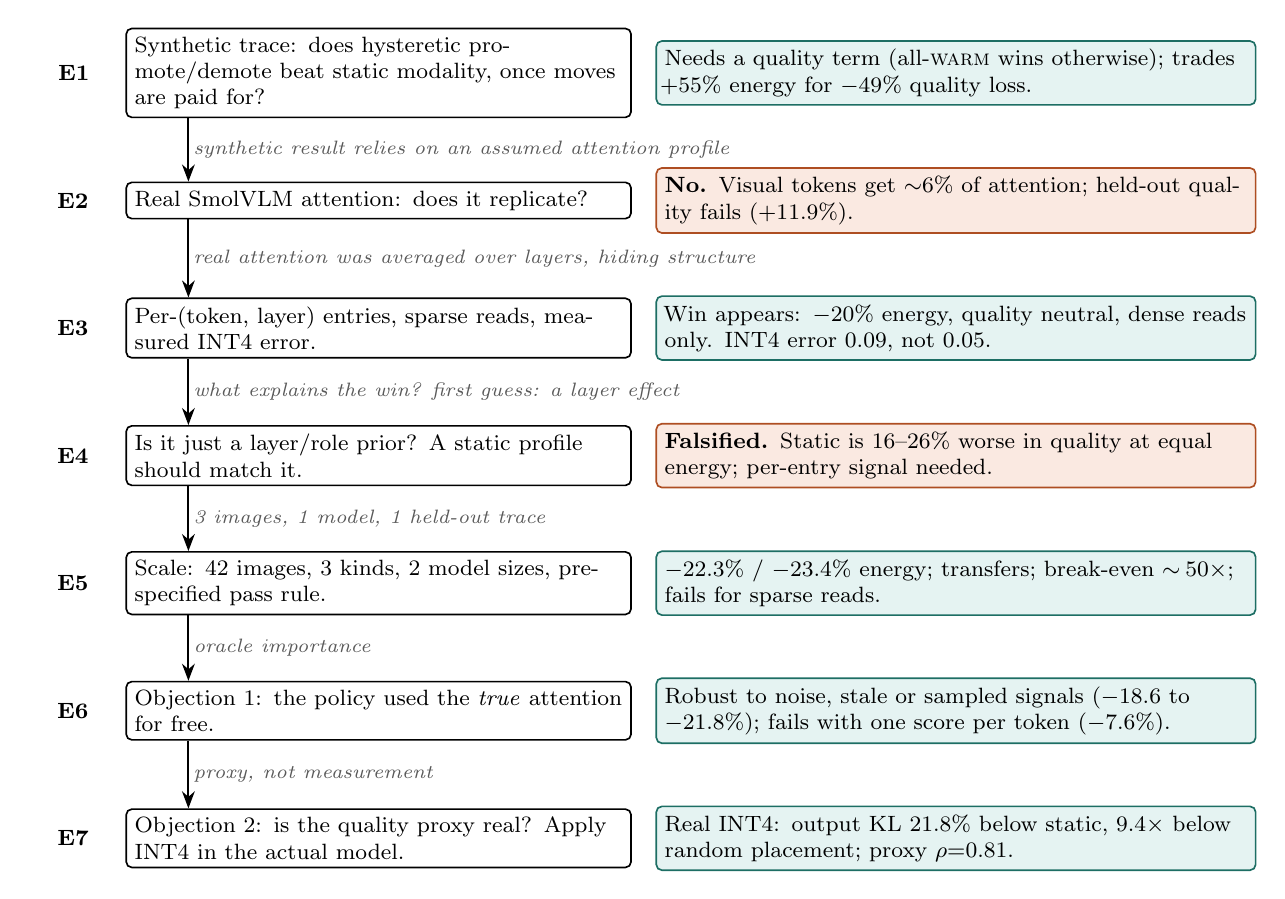
\begin{tikzpicture}[font=\footnotesize, >=Stealth,
  q/.style={draw, rounded corners=2pt, text width=62mm, align=left, inner sep=3pt, fill=white, line width=0.6pt},
  f/.style={draw, rounded corners=2pt, text width=74mm, align=left, inner sep=3pt, line width=0.6pt},
  tag/.style={font=\bfseries\footnotesize, text width=9mm, align=center},
  nx/.style={font=\scriptsize\itshape, text=black!65, text width=95mm, align=left}]
\def\dy{-16.2mm}
\node[tag] (t1) at (0,0) {E1};
\node[q, right=1mm of t1, anchor=west] (q1) {Synthetic trace: does hysteretic promote/demote beat static modality, once moves are paid for?};
\node[f, right=3mm of q1, fill=okc!12, draw=okc!70!black] (f1) {Needs a quality term (all-\warm{} wins otherwise); trades $+55\%$ energy for $-49\%$ quality loss.};
\node[tag] (t2) at (0,\dy) {E2};
\node[q, right=1mm of t2, anchor=west] (q2) {Real SmolVLM attention: does it replicate?};
\node[f, right=3mm of q2, fill=hotc!14, draw=hotc!80!black] (f2) {\textbf{No.} Visual tokens get $\sim$6\% of attention; held-out quality fails ($+11.9\%$).};
\node[tag] (t3) at (0,2*\dy) {E3};
\node[q, right=1mm of t3, anchor=west] (q3) {Per-(token, layer) entries, sparse reads, measured INT4 error.};
\node[f, right=3mm of q3, fill=okc!12, draw=okc!70!black] (f3) {Win appears: $-20\%$ energy, quality neutral, dense reads only. INT4 error $0.09$, not $0.05$.};
\node[tag] (t4) at (0,3*\dy) {E4};
\node[q, right=1mm of t4, anchor=west] (q4) {Is it just a layer/role prior? A static profile should match it.};
\node[f, right=3mm of q4, fill=hotc!14, draw=hotc!80!black] (f4) {\textbf{Falsified.} Static is $16$--$26\%$ worse in quality at equal energy; per-entry signal needed.};
\node[tag] (t5) at (0,4*\dy) {E5};
\node[q, right=1mm of t5, anchor=west] (q5) {Scale: 42 images, 3 kinds, 2 model sizes, pre-specified pass rule.};
\node[f, right=3mm of q5, fill=okc!12, draw=okc!70!black] (f5) {$-22.3\%$ / $-23.4\%$ energy; transfers; break-even $\sim\!50\times$; fails for sparse reads.};
\node[tag] (t6) at (0,5*\dy) {E6};
\node[q, right=1mm of t6, anchor=west] (q6) {Objection 1: the policy used the \emph{true} attention for free.};
\node[f, right=3mm of q6, fill=okc!12, draw=okc!70!black] (f6) {Robust to noise, stale or sampled signals ($-18.6$ to $-21.8\%$); fails with one score per token ($-7.6\%$).};
\node[tag] (t7) at (0,6*\dy) {E7};
\node[q, right=1mm of t7, anchor=west] (q7) {Objection 2: is the quality proxy real? Apply INT4 in the actual model.};
\node[f, right=3mm of q7, fill=okc!12, draw=okc!70!black] (f7) {Real INT4: output KL $21.8\%$ below static, $9.4\times$ below random placement; proxy $\rho{=}0.81$.};
\foreach \a/\b/\txt in {1/2/{synthetic result relies on an assumed attention profile},2/3/{real attention was averaged over layers, hiding structure},3/4/{what explains the win? first guess: a layer effect},4/5/{3 images, 1 model, 1 held-out trace},5/6/{oracle importance},6/7/{proxy, not measurement}}{
  \draw[->, line width=0.7pt] ($(q\a.south west)+(8mm,0)$) -- node[right=1pt, font=\scriptsize\itshape, text=black!65, inner sep=0.5pt] {\txt} ($(q\b.north west)+(8mm,0)$);}
\end{tikzpicture}

\caption{The study as a chain of hypotheses. Each box states the question, the finding, and (on the arrow) the weakness that forced the next experiment. Red marks results that overturned an earlier belief (E2, E4) or missed a pre-specified criterion (E9).}
\label{fig:roadmap}
\end{figure}

\section{Related Work}
\paragraph{Algorithm-level visual KV compression.} VL-Cache~\cite{vlcache} (modality- and sparsity-aware budgeting), ZipVL~\cite{zipvl} (dynamic token sparsification), AirCache~\cite{aircache} and TopV~\cite{topv} (inter-modal relevance and token pruning) and FastV~\cite{fastv} (early-layer visual token pruning) show that visual tokens are, on average, less important to decoding than text tokens and can be compressed with small accuracy loss. For text LLMs, H2O~\cite{h2o} and SnapKV~\cite{snapkv} keep heavy-hitter entries, StreamingLLM~\cite{streaming} keeps attention sinks plus a recent window, KIVI~\cite{kivi} quantizes the cache to 2 bits, and Quest~\cite{quest} reads only query-relevant pages. These methods \emph{discard or shrink}. We instead ask where an entry should reside and what it costs to move it, a question they do not pose because their memory is flat.

\paragraph{Memory-centric and in-memory computing.} The case for computing where the data is, because moving data dominates energy, is made in the processing-in-memory literature~\cite{mutlu19}, and commercial DRAM-based PIM exists~\cite{hbmpim}. Recent proposals place the attention stage of LLM decoding on in-/near-memory units~\cite{attacc,neupims}. We do not compare against these designs. Our question is the runtime one they leave open in the setting we study: given data whose importance and reuse change during execution, and in-memory units that are finite and lossy, \emph{which data should be resident where, which reads should run in memory, and what do the observation and migration cost?}

\paragraph{Memory systems for LLM serving.} PagedAttention~\cite{vllm} manages KV memory in fixed blocks. Our contribution is orthogonal: a migration-cost model for \emph{moving} entries between a high-fidelity tier and a low-energy lossy tier, a compute-site scheduler, and an evaluation on real attention under three access regimes, with the conditions under which dynamic placement fails.

\paragraph{Positioning.} Our access-cost constants are stylised ratios (Table~\ref{tab:tiers}), not a specific device, so absolute energies are not claims about hardware. What the study can support are \emph{ratios between policies under one shared cost model} and the sensitivity of those ratios to the assumptions that matter.

\section{System Model}
\subsection{Entities and tiers}
A decode session has a prefill of $n_p$ tokens (visual or text) followed by $T{=}64$ generated tokens. Following the per-layer view of Sec.~\ref{sec:layers}, one \emph{entry} is the KV pair of one (token, layer); a model with $\ell$ layers has $\ell$ entries per token. Every decode step, every active entry is read once (dense reads) with attention weight $w_{e,t}$, $\sum_e w_{e,t}{=}1$.

\begin{figure}[t]
\centering
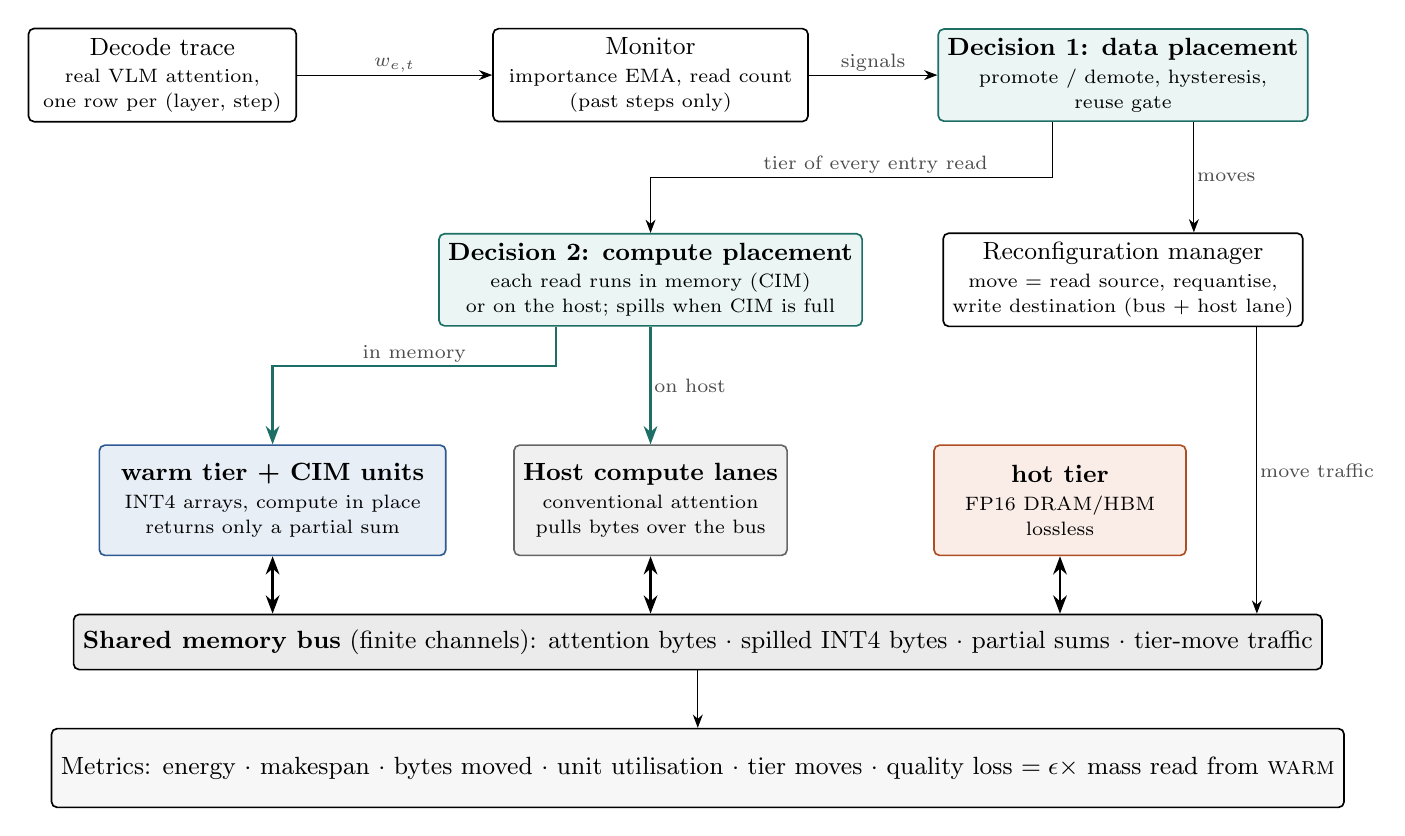
\begin{tikzpicture}[font=\small, >=Stealth,
  box/.style={draw, rounded corners=2pt, minimum height=10mm, align=center, fill=white, line width=0.6pt},
  dec/.style={box, fill=okc!10, draw=okc!70!black},
  hotb/.style={box, fill=hotc!12, draw=hotc!80!black, minimum height=14mm},
  warmb/.style={box, fill=warmc!12, draw=warmc!80!black, minimum height=14mm},
  hostb/.style={box, fill=black!6, draw=black!60, minimum height=14mm},
  lab/.style={font=\scriptsize, text=black!70, align=center, fill=white, inner sep=1pt}]
% runtime: observe, then two decisions
\node[box, minimum width=34mm] (trace) at (0,0) {Decode trace\\[-1pt]{\scriptsize real VLM attention,}\\[-2pt]{\scriptsize one row per (layer, step)}};
\node[box, minimum width=40mm] (mon) at (6.2,0) {Monitor\\[-1pt]{\scriptsize importance EMA, read count}\\[-2pt]{\scriptsize (past steps only)}};
\node[dec, minimum width=44mm] (pol) at (12.2,0) {\textbf{Decision 1: data placement}\\[-1pt]{\scriptsize promote / demote, hysteresis,}\\[-2pt]{\scriptsize reuse gate}};
\node[dec, minimum width=42mm] (sched) at (6.2,-2.6) {\textbf{Decision 2: compute placement}\\[-1pt]{\scriptsize each read runs in memory (CIM)}\\[-2pt]{\scriptsize or on the host; spills when CIM is full}};
\node[box, minimum width=44mm] (rec) at (12.2,-2.6) {Reconfiguration manager\\[-1pt]{\scriptsize move = read source, requantise,}\\[-2pt]{\scriptsize write destination (bus + host lane)}};
% resources
\node[warmb, minimum width=44mm] (warm) at (1.4,-5.4) {\textbf{\warm{} tier + CIM units}\\[-1pt]{\scriptsize INT4 arrays, compute in place}\\[-2pt]{\scriptsize returns only a partial sum}};
\node[hostb, minimum width=30mm] (host) at (6.2,-5.4) {\textbf{Host compute lanes}\\[-1pt]{\scriptsize conventional attention}\\[-2pt]{\scriptsize pulls bytes over the bus}};
\node[hotb, minimum width=32mm] (hot) at (11.4,-5.4) {\textbf{\hot{} tier}\\[-1pt]{\scriptsize FP16 DRAM/HBM}\\[-2pt]{\scriptsize lossless}};
\node[box, minimum width=156mm, minimum height=7mm, fill=black!8] (bus) at (6.8,-7.2) {\textbf{Shared memory bus} (finite channels): attention bytes $\cdot$ spilled INT4 bytes $\cdot$ partial sums $\cdot$ tier-move traffic};
\node[box, minimum width=120mm, fill=black!3] (met) at (6.8,-8.8) {Metrics: energy $\cdot$ makespan $\cdot$ bytes moved $\cdot$ unit utilisation $\cdot$ tier moves $\cdot$ quality loss $=\epsilon\times$ mass read from \warm{}};
\draw[->] (trace) -- (mon) node[midway, above, lab]{$w_{e,t}$};
\draw[->] (mon) -- (pol) node[midway, above, lab]{signals};
\draw[->] ([xshift=-9mm]pol.south) -- ++(0,-7mm) -| (sched.north) node[pos=0.22, above, lab]{tier of every entry read};
\draw[->] ([xshift=9mm]pol.south) -- ([xshift=9mm]rec.north) node[midway, right, lab]{moves};
\draw[->, line width=0.8pt, okc!70!black] (sched.south) -- (host.north) node[midway, right, lab]{on host};
\draw[->, line width=0.8pt, okc!70!black] ([xshift=-12mm]sched.south) -- ++(0,-5mm) -| (warm.north) node[pos=0.25, above, lab]{in memory};
\draw[->] ([xshift=17mm]rec.south) -- ([xshift=17mm]rec.south |- bus.north) node[pos=0.5, right, lab]{move traffic};
\draw[<->, line width=0.8pt] (warm.south) -- (warm.south |- bus.north);
\draw[<->, line width=0.8pt] (host.south) -- (host.south |- bus.north);
\draw[<->, line width=0.8pt] (hot.south) -- (hot.south |- bus.north);
\draw[->] (bus.south) -- (met.north);
\end{tikzpicture}

\caption{System model. A decode trace supplies, per step, the attention each entry receives. The monitor (past steps only) tracks importance and read counts. Two runtime decisions follow: where each entry's data lives (tier; changed by migrations, which are priced as bus and host-lane traffic) and where each read is computed (in \warm{}'s CIM units, or on the host after pulling the bytes over the bus). All reads, partial sums and migrations share the finite bus; quality is accounted separately from energy and latency.}
\label{fig:arch}
\end{figure}

\begin{table}[t]
\centering\small
\caption{Tier cost model (stylised, one shared set of ratios for all policies). The per-access cost is $c_0 + c_1\cdot\text{bytes}$ at the tier's own precision.}
\label{tab:tiers}
\begin{tabular}{lccccc}
\toprule
Tier & Precision & Base lat. (ns) & Lat./byte (ns) & Base energy (pJ) & Energy/byte (pJ)\\
\midrule
\hot{}  & FP16 (2 B/elem) & 20 & 0.010 & 5.0 & 8.0\\
\warm{} & INT4 (0.5 B/elem) & 30 & 0.015 & 0.5 & 0.8\\
\bottomrule
\end{tabular}
\\[2pt]
{\footnotesize \warm{} is $10\times$ cheaper per byte in energy, $1.5\times$ slower per access, and stores 4$\times$ fewer bytes. Quality weight of a \warm{} read: INT4 relative error $\epsilon$.}
\end{table}

\subsection{Quality proxy}
Reading entry $e$ from \warm{} perturbs its key and value by INT4 quantization. We charge a quality loss of $w_{e,t}\cdot\epsilon$, so the per-step quality loss is $\epsilon$ times the attention mass served from \warm{}. The simulator's default is $\epsilon{=}0.05$, an assumption made before any measurement. We later measured $\epsilon$ on real SmolVLM KV tensors (per-token asymmetric min-max INT4, groups of 32): relative $L_2$ error $0.102$ (K) and $0.081$ (V), about $0.09$ on average and $\sim\!1.8\times$ our default; visual and text tokens differ by under 1\%. Because loss is linear in $\epsilon$, \emph{every quality ratio between policies is unchanged}, and only absolute quality values scale. Section~\ref{sec:real} tests whether this proxy actually predicts the real model's behaviour.

\subsection{Importance monitor and policy}
The monitor keeps an exponential moving average (EMA, decay $0.9$) of the attention each entry receives, updated at the end of every step from that step's weights only. The \emph{dynamic hybrid} policy starts each entry at its modality prior (visual $\rightarrow$ \warm{}, text $\rightarrow$ \hot{}) and then applies a hysteresis rule: promote \warm{}$\to$\hot{} when importance exceeds $\theta_{\uparrow}$ and demote \hot{}$\to$\warm{} when it falls below $\theta_{\downarrow}<\theta_{\uparrow}$. A warm-up of two EMA updates prevents moves driven by the zero-initialised EMA. Thresholds are expressed in multiples of \emph{uniform attention} $1/n_p$ (so a threshold of $8\times$ means ``eight times what a uniform cache would give each entry''), which makes them comparable across traces of different length.

\subsection{Reconfiguration and its linearity}
A tier change costs $m$ times one \hot{} access, in both latency and energy ($m{=}10$ by default). Policy decisions depend on the importance EMA and never on cost, so a run's totals decompose exactly as
\begin{equation}
E(m)=E_{\text{access}}+m\,E_{\text{reconf}}^{(1\times)},
\end{equation}
which is verified by a unit test. We therefore simulate once at $m{=}1$ and obtain any other cost as an exact post-hoc sum. This is what makes the cost sweeps in Sec.~\ref{sec:scale} cheap and exact (thresholds are, however, \emph{re-selected} at each cost).

\subsection{Baselines and metrics}
\textbf{Flat}: everything in \hot{}. \textbf{Static modality}: visual in \warm{}, text in \hot{}, never moved; this is the strong baseline throughout and all results are percentages \emph{relative to it}, per trace. \textbf{Static layer/role profile}: groups of (modality or role) $\times$ layer placed in \hot{} when their mean importance exceeds a threshold, fixed offline (Sec.~\ref{sec:m6b}). We report total energy, serialised latency, the quality proxy, and the number of tier moves. \textbf{Sparse reads} (Sec.~\ref{sec:layers}) read only the top-$k\%$ entries by live importance plus entries created in the last step.

\subsection{Compute resources, data movement and runtime scheduling (system model)}
\label{sec:sys}
Experiments E1--E7 use the access-cost model above: the tier implies the compute site, latencies are summed serially and a migration is a lump-sum multiple of a \hot{} access. That isolates the data-placement question but cannot show contention, data movement or a choice of compute site. E8--E9 therefore use a second model (\texttt{system.py}; the first simulator is untouched so E1--E7 stay reproducible) in which resources are explicit and shared (Fig.~\ref{fig:arch}, Tab.~\ref{tab:sys}).

\begin{table}[t]
\centering\small
\caption{System model parameters (defaults used in E8--E9 unless a sweep says otherwise). Tier access costs are those of Tab.~\ref{tab:tiers}.}
\label{tab:sys}
\begin{tabular}{>{\raggedright\arraybackslash}p{3.6cm}>{\raggedright\arraybackslash}p{11.8cm}}
\toprule
Element & Model\\
\midrule
Resources & 8 memory-bus channels, 8 host compute lanes, 16 CIM units (swept 2--64 in E8). Work is issued as packets of 64 entries; a packet occupies one unit of a resource at a time and queues FIFO.\\
\hot{} read (host) & occupies a bus channel for the \hot{} access latency (movement), then a host lane for 2 ns/entry (MACs). Energy: \hot{} access energy.\\
\warm{} read in memory & occupies a CIM unit for the \warm{} access latency; returns a 32 B partial sum per packet over the bus. Energy: \warm{} access energy plus the partial-sum transfer.\\
\warm{} read on host (``spill'') & pulls the INT4 bytes over the bus at the \hot{}-path cost, then dequantises (1 ns, 10 pJ/entry) and computes on a host lane. The data stay INT4, so the quality loss is the same.\\
Scheduler & \texttt{tier}: \warm{} reads run in memory; \texttt{host}: \warm{} is compressed storage only; \texttt{adaptive}: each \warm{} packet goes where the estimated finish time (from the work already assigned in this step) is earlier.\\
Tier move (migration) & reads the source tier, requantises and updates metadata (14 ns on a host lane, 60 pJ) and writes the destination tier, all over the bus. This bottom-up cost is $\approx\!1.05\times$ one \hot{} access, versus the $10\times$ assumed in E1--E7; \texttt{reconfig\_scale} scales it.\\
Step semantics & Reads of a step are issued together and the step ends at the last packet (a barrier); moves are then issued and also complete before the next step. Energy is additive; latency is the makespan.\\
\bottomrule
\end{tabular}
\end{table}

\paragraph{Regression anchor.} With one global server, no compute time, no partial-sum traffic and the lump-sum migration cost, the model reproduces the first simulator's energy, latency, quality and move counts to $10^{-9}$ relative error for the flat, static and dynamic policies (unit test). Everything new is therefore an addition, not a re-parameterisation.

\paragraph{Access regimes.} The attention weights are always the real ones; a regime says which entries are \emph{read}. \emph{Reusable}: all active entries every step (as in all earlier experiments). \emph{Streaming}: the prefill is consumed once, in order, $\lceil n_p^{\text{tok}}/T\rceil$ tokens per step, plus the newest token, so every entry is read once. \emph{Random}: a uniformly random 3\%, 10\% or 30\% of entries per step, redrawn each step, plus the newest token. Weight on unread entries is reported as skipped mass (identical for all placement policies, so comparisons within a regime are fair). The monitor sees only what is read: an unread entry's importance is not updated. These regimes are access-pattern \emph{overlays} on real attention, not separate real workloads, which we list as a limitation.

\paragraph{Reuse-aware placement.} The runtime counts how often an entry was read ($\text{reuse}=\text{reads}/\text{age}$). A migration of cost $R$ that saves $G$ per read repays only if the entry is read at least $R/G$ more times; $R/G$ is computed from the cost model (1.08 reads at the bottom-up cost, 10.8 at $10\times$ that). The \emph{reuse-aware} policy is the dynamic policy with moves suppressed unless $\text{reuse}\times 32\ \text{steps}\ge R/G$. With dense reads $\text{reuse}=1$ and it is identical to the dynamic policy (unit test).

\section{Evaluation Protocol}
\label{sec:protocol}
Because the policy has free thresholds, the main risk is fitting them to the test set. We adopted three rules and kept them across milestones.
\begin{enumerate}[leftmargin=1.3em]
\item \textbf{Selection rule.} Thresholds $(\theta_\uparrow,\theta_\downarrow)$ are the pair with the lowest mean energy among those whose mean quality loss is no worse than static modality's on the \emph{training} traces (fallback: lowest quality loss).
\item \textbf{Held-out evaluation.} Milestone 5--6: fit on two traces, test on the third. Milestone 7--8: \emph{leave-one-trace-out} over all 42 traces. Results are held-out means.
\item \textbf{A fixed pass criterion for the headline claim} (written before the 42-image runs; for E8--E9 the hypotheses H8a--H9e and their criteria were written in the lab notes after the runs were launched but before any result was inspected, Tab.~\ref{tab:score}): mean held-out energy saving $\ge 10\%$; mean quality-loss change $\le +2\%$; paired-bootstrap 95\% CI of the energy saving excludes 0; the sign holds in each of the three image kinds. Anything weaker is reported as ``not established''.
\end{enumerate}
Deviations from pre-set plans are stated where they occur: the choice of damping rule (Sec.~\ref{sec:synth}), the change of thresholds to multiples of uniform attention after the first real-data failure (Sec.~\ref{sec:real5}), the widening of the threshold grid after every fold chose the grid corner (Sec.~\ref{sec:scale}), and the minimum-age variant of the reuse gate, added after H9c failed and labelled post hoc (Sec.~\ref{sec:e9}). E8--E9 do not re-tune thresholds: the E5 choice ($8\times/0.4\times$) is used throughout.

\paragraph{Data.} Three locally generated images (chart, scene, noise+label) for Milestones 5--6; 42 images for Milestone 7--8 (24 COCO val2017 photos~\cite{coco}, 10 matplotlib charts, 8 rendered text documents), each with a task prompt. Models: SmolVLM-256M-Instruct (primary) and SmolVLM-500M-Instruct~\cite{smolvlm}. Per image, we greedy-decode 64 tokens and record, at every step, the head-averaged attention row of every layer (30 layers for 256M). The generated text was checked to confirm the model uses the image.

\section{Experiments, in the Order They Built on One Another}
The first seven experiments (E1--E7) use the access-cost model of Sec.~3 (the tier implies the compute site; latency is serialised) and ask where \emph{data} should live. E8--E9 use the system model of Sec.~\ref{sec:sys} and ask where \emph{computation} should run and how the answer depends on data reuse.

\subsection{E1 --- Synthetic traces: is dynamic placement worth its reconfiguration cost?}
\label{sec:synth}
\textbf{Question.} Does a hysteretic promote/demote policy beat static modality tiering once moves are paid for? \textbf{Setup.} A synthetic trace (20 text + 500 visual tokens, 64 steps, a salient 8\% of visual tokens, recency bias) reproduces the literature's pattern that visual tokens are on average less important but a salient minority persists.

\textbf{Step 1: an energy-and-latency-only comparison is degenerate.} A trivial \emph{all-\warm{}} policy beat every dynamic configuration by $-78.6\%$ energy at $+2.6\%$ latency. With no cost for INT4 error, \hot{} has no reason to exist. We added the quality term of Sec.~3.2.

\textbf{Step 2: the policy trades energy for quality.} With quality included, the first dynamic policy \emph{lost} to static modality ($+67\%$ energy): recency-driven importance spikes at the prefill/decode boundary promoted entries that fell back below the demote threshold within $\sim$20 steps, so entries round-tripped and each round trip cost $10\times$ a \hot{} access. Adding a 2-step warm-up (selected over alternatives by quality gain per unit of energy, a post-hoc choice we record as such) cut energy overhead from $+64.8\%$ to $+55.8\%$ and improved quality from $-46.1\%$ to $-49.3\%$; a longer dwell time only batched all moves into one burst.

\begin{figure}[t]
\centering
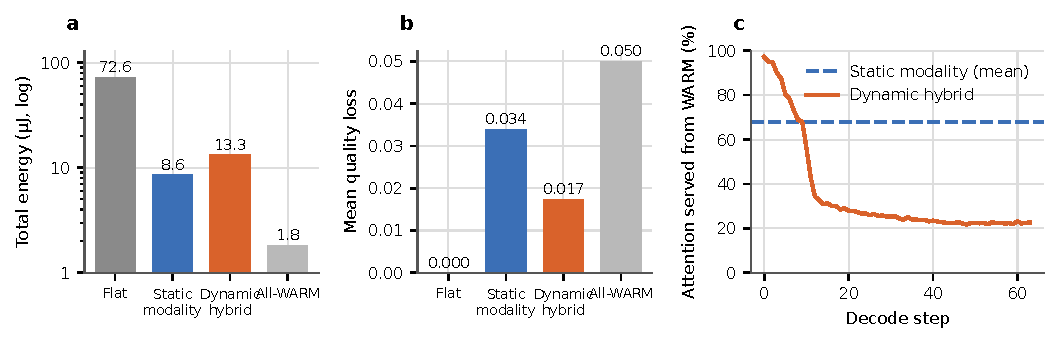
\includegraphics[width=\linewidth]{figs/fig_synth.pdf}
\caption{Synthetic trace, default configuration, $10\times$ reconfiguration cost. (a, b) The dynamic policy sits between static modality and flat on energy and halves the quality loss. (c) It does so by promoting the salient visual tokens in the first $\sim$12 steps, cutting the attention mass served from \warm{} from $\sim$97\% to $\sim$36\% by step 12 and $\sim$25\% by the end.}
\label{fig:synth}
\end{figure}

\textbf{Finding.} On the synthetic trace, dynamic placement buys a large \emph{quality} gain ($-48.8\%$ quality loss) for $+55\%$ energy over static modality (Fig.~\ref{fig:synth}), a far better rate than interpolating between static and flat (flat: $-100\%$ quality loss for $+748\%$ energy). \textbf{Limitation that drives E2.} This depends on 68\% of attention mass landing on \warm{}-resident salient visual tokens, an assumption of the generator. Whether real VLMs behave this way was untested.

\subsection{E2 --- Real attention: does the synthetic result replicate?}
\label{sec:real5}
\textbf{Question.} Replace the generator by SmolVLM-256M's measured decode attention (3 images, layer- and head-averaged, one entry per token). \textbf{Finding: it does not replicate.} Visual tokens receive only $\sim$6\% of the attention mass ($5$--$7\%$ across the three images), versus 68\% served from \warm{} in the synthetic trace. A single attention sink at position 0 takes $\sim$35\%, and recently generated tokens another $\sim$36\% (Fig.~\ref{fig:anatomy}a). The visual attention that exists is heavy-tailed and persistent as assumed (the top 8\% of visual tokens hold 61--70\% of visual mass, with a 74--83\% overlap between the first and last step), but the stakes are small: static modality already sits near the quality floor (quality loss $\approx$0.003), so flat$\to$static is $-88$ to $-90\%$ energy for almost no quality.

\begin{figure}[t]
\centering
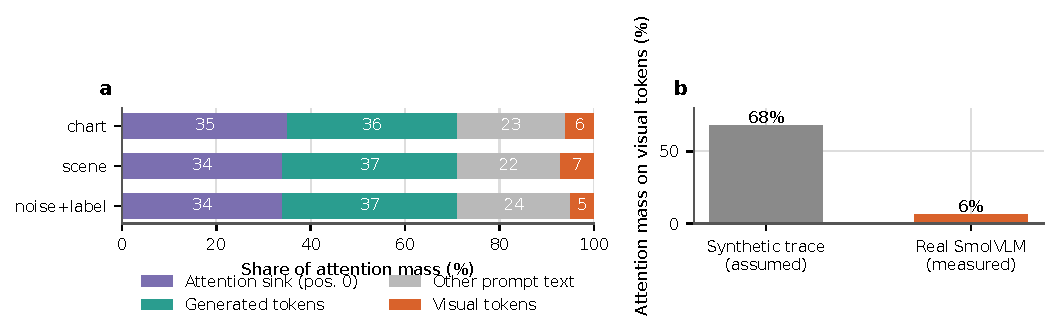
\includegraphics[width=\linewidth]{figs/fig_anatomy.pdf}
\caption{(a) Where real decode attention goes (SmolVLM-256M, three images; layer- and head-averaged). (b) The synthetic trace badly overstated how much attention the \warm{} tier would serve.}
\label{fig:anatomy}
\end{figure}

\textbf{A second failure: synthetic thresholds do not transfer.} Uniform attention is $\approx$0.0011 and even the 99th-percentile visual EMA ($\approx$0.0008) is below the synthetic promote threshold (0.006), so nothing visual is ever promoted; the policy then only demotes text, with $-23$ to $-27\%$ energy but $+37$ to $+42\%$ quality loss. Re-expressing thresholds in multiples of uniform attention (a deviation we record) and following the protocol of Sec.~\ref{sec:protocol} (fit on two traces, test on the third) gave thresholds $2.0\times/0.4\times$ and, on the held-out trace, $-14.4\%$ energy but $+11.9\%$ quality loss: the no-worse-quality criterion \textbf{failed}. \textbf{Conclusion of E2:} the M4 trade-off was a property of the synthetic trace. We kept the negative result and asked what the layer- and head-averaging was hiding. A per-layer look at one trace shows visual attention mass varying from $\sim$3\% to 39\% across layers (layer 0: 39\%) and the sink being $\approx$0\% in layers 0--1 but 40--78\% in layers 12--30, so one averaged entry per token plausibly hid the structure a policy could use.

\subsection{E3 --- Per-(token, layer) entries, sparse reads, and measured INT4 error}
\label{sec:layers}
\textbf{Changes.} (i) One entry per (token, layer), with each layer's attention renormalised so the step's total mass stays 1; (ii) a \emph{sparse-read} model (top-$k\%$ entries by live importance plus the newest entries; skipped mass is reported and costs nothing; the importance estimate is an upper bound, oracle and free); (iii) a measured INT4 error (Sec.~3.2). Same protocol as E2.

\begin{table}[t]
\centering\small
\caption{E3: held-out trace (fit on the other two), dynamic vs static modality, $10\times$ reconfiguration cost. ``Layer-avg'' is E2's single entry per token.}
\label{tab:e3}
\begin{tabular}{lcccc}
\toprule
Entries / reads & Flat/static energy & Chosen $\theta_\uparrow/\theta_\downarrow$ & Energy & Quality loss\\
\midrule
Layer-avg, dense        & 9.3$\times$ & 2.0/0.4 & $-14.4\%$ & $+11.9\%$\\
Layer-avg, top-10\%     & 1.6$\times$ & 8.0/0.02 & $+0.2\%$ (no moves) & $0\%$\\
Per-layer, dense        & 9.3$\times$ & 4.0/0.4 & $\mathbf{-20.0\%}$ & $+0.8\%$\\
Per-layer, top-10\%     & 1.9--2.0$\times$ & 8.0/0.2 & $+3.7\%$ & $-0.2\%$\\
\bottomrule
\end{tabular}
\end{table}

\textbf{Finding: the first real-data win.} With per-layer entries and dense reads the dynamic policy saves $\sim$20\% energy on all three traces ($-20.6/-19.4/-20.0\%$) at roughly neutral quality ($-2.0/-10.3/+0.8\%$), using 1.2--1.4k tier moves per session (Tab.~\ref{tab:e3}). The held-out quality ($+0.8\%$) technically misses the strict ``no worse than static'' rule, which we state rather than round. Two boundary results appear: sparse reads shrink the headroom from $\sim\!9.3\times$ to $\sim\!1.6$--$2\times$ and the dynamic policy either has nothing to do (layer-average) or loses (per-layer, $+3.7$ to $+7.5\%$): with sparse reads \hot{} text entries are rarely read, so demoting them saves little while the moves still cost.

\textbf{What this left open.} (a) An explanation: our working hypothesis was a \emph{layer effect}. (b) $n=3$ images, one model, one held-out trace.

\subsection{E4 --- Is the per-layer win merely a layer prior? A falsification test}
\label{sec:m6b}
\textbf{Hypothesis (stated before testing).} If the win is a layer effect, a \emph{static} profile, a group importance map by (modality, layer) or (role, layer) with $\text{role}\in\{$sink, prompt text, generated, visual$\}$ built offline and with zero moves, should capture it. \textbf{Protocol.} Leave-one-trace-out profile and threshold $\theta$ (eight values from 0.05 to 4.0), plus an in-sample ceiling.

\begin{figure}[t]
\centering
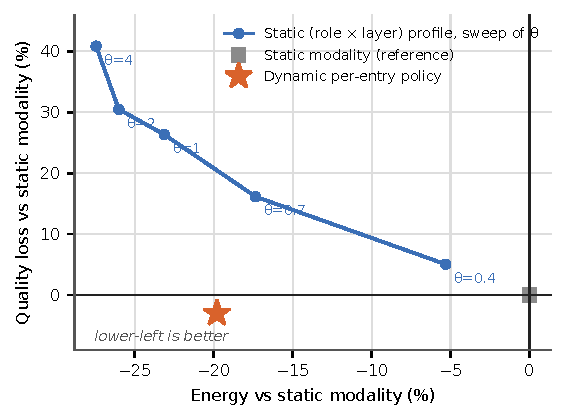
\includegraphics[width=0.5\linewidth]{figs/fig_m6b.pdf}\hfill
\begin{minipage}[b]{0.46\linewidth}
\caption{E4: the static (role $\times$ layer) profile traces a trade-off curve (dense reads, mean of three held-out folds) and never reaches the dynamic policy. At matched energy ($\approx-20\%$) the static profile loses roughly 16--26\% in quality while the dynamic policy gains 3\%.}
\label{fig:m6b}
\end{minipage}
\end{figure}

\textbf{Finding: hypothesis falsified.} At matched energy, the static profile has clearly worse quality than the dynamic policy (Fig.~\ref{fig:m6b}). The (modality, layer) grouping is degenerate (for $\theta\ge0.4$ it selects exactly the text groups, i.e.\ static modality), and the in-sample ceiling ($+27.2\%$ energy, $-18.4\%$ quality) nearly equals the cross-validated result ($+27.7\%$, $-18.6\%$), so this is neither under-fitting nor leakage: layer- and role-level information is too coarse. \textbf{Correction.} We had written that the saving came from ``demoting text entries in layers where text is unimportant''. The arithmetic stands (text entries are $\sim$45\% of static energy and the saving is about half of that) but the \emph{layer} part was wrong: no text layer group is unimportant on average. The saving comes from variation among individual text entries, i.e.\ which prompt tokens matter in this prompt, which only a per-entry, online signal sees. \textbf{What this left open:} everything rests on three images and one model.

\subsection{E5 --- Scale-up: 42 images, three image kinds, two model sizes}
\label{sec:scale}
\textbf{Pre-specified claims} (fixed before running; Sec.~\ref{sec:protocol}): (a) the dense-read win holds under leave-one-trace-out; (b) its dependence on the reconfiguration cost; (c) its dependence on sparse read fraction; (d) transfer to a larger model (256M thresholds applied unchanged to 500M). Min-dwell variants were an additional check on move count.

\begin{table}[t]
\centering\small
\caption{E5, dense reads, $10\times$ reconfiguration cost, leave-one-trace-out over 42 images. Percentages are vs static modality, per trace, then averaged; brackets are paired-bootstrap 95\% CIs. Quality loss $<0$ is better.}
\label{tab:e5}
\begin{tabular}{lcccc}
\toprule
Setting & Energy & Quality loss & Selected $\theta_\uparrow/\theta_\downarrow$ & Passes criterion\\
\midrule
256M, leave-one-out       & $-22.3\%$ [$-22.8,-21.9$] & $-2.5\%$ [$-4.0,-1.1$] & 8/0.4 (42/42 folds) & yes\\
500M, leave-one-out       & $-23.4\%$ [$-24.1,-22.6$] & $-1.8\%$ [$-4.6,+0.9$] & 4/0.8 (42/42) & yes\\
256M thresholds $\to$ 500M & $-23.6\%$ [$-24.1,-23.1$] & $+0.4\%$ [$-1.4,+2.1$] & 8/0.4 (no refit) & yes\\
\midrule
256M, top-10\% reads      & $+5.7\%$ [$+5.4,+5.9$] & $-0.7\%$ & 32/0.02 & \textbf{no}\\
500M, top-10\% reads      & $+5.7\%$ [$+5.4,+6.0$] & $-0.6\%$ & 32/0.02 & \textbf{no}\\
\bottomrule
\end{tabular}
\end{table}

\textbf{(a) The win is robust for dense reads.} The saving is negative on every one of the 42 traces. By image kind (256M): charts $-22.8\%$, documents $-20.2\%$, natural photos $-22.9\%$. Quality is \emph{neutral, not improved}: the per-trace rate of ``energy down and quality no worse'' is 76\% on 256M and 55\% on 500M, and the 500M quality interval includes zero. The ladder of Fig.~\ref{fig:ladder} shows how the estimate moved from E2 to here.

\begin{figure}[t]
\centering
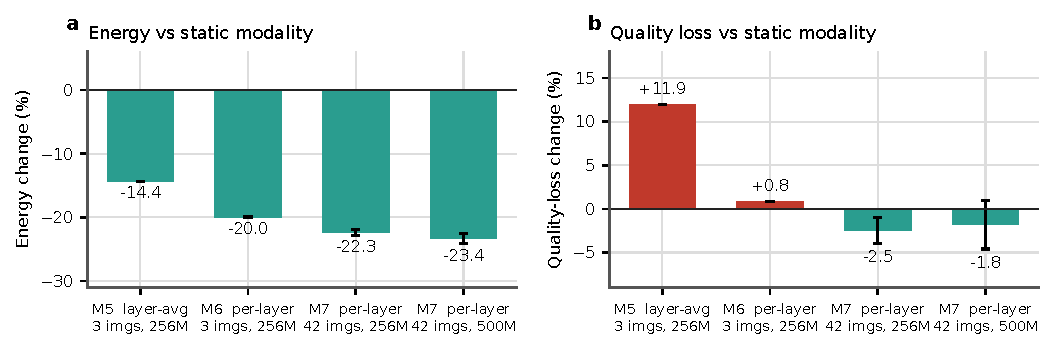
\includegraphics[width=\linewidth]{figs/fig_ladder.pdf}
\caption{Held-out effect of the dynamic policy across the stages of the study. The first bar is E2 (single entry per token), the second E3 (per layer); the last two are E5. Error bars are 95\% CIs (not available for the 3-trace stages).}
\label{fig:ladder}
\end{figure}

\textbf{Grid edge.} The first 256M pass selected the grid corner (promote $8\times$, demote $0.4\times$) in all 42 folds, which would make leave-one-out meaningless and suggested the optimum might lie outside the grid. We widened the grid (promote up to $32\times$, demote up to $1.6\times$) after seeing this and re-ran (first-pass results are kept). The 10$\times$ dense result \emph{did not change} (still $-22.3\%$, 8/0.4 in all folds): the corner was a real optimum and not a search limit.

\textbf{(b) Reconfiguration cost.} Re-selecting thresholds at each cost, the saving is $-31.6\%$ at $1\times$, $-26.5\%$ at $5\times$, $-16.1\%$ at $20\times$, $-1.7\%$ at $50\times$ and $+13.4\%$ at $100\times$ on 256M (500M: $-32.3, -27.7, -15.1, -1.9, +13.2$). The break-even is about $50\times$ on both models, leaving a factor of about five of margin at the default $10\times$ (Fig.~\ref{fig:cost}a). \textbf{(c) Sparse reads.} With top-10\% reads the dynamic policy \emph{loses} ($+5.7\%$ energy on both models, every trace worse). The 256M sweep over read fraction gives $-20.1\%$ (top-50\%), $-6.0\%$ (top-20\%), $+7.5\%$ (top-10\%) and $+15.0\%$ (top-5\%) (Fig.~\ref{fig:cost}b): the advantage needs dense or nearly dense reads. The chosen thresholds at 10\% (32/0.02) sit at a new grid corner, so we cannot exclude a modest shift with a wider grid, but not a change of sign of this magnitude. \textbf{(d) Transfer.} 256M thresholds applied unchanged to 500M give $-23.6\%$ energy at $+0.4\%$ quality, essentially the same as 500M's own cross-validated optimum.

\begin{figure}[t]
\centering
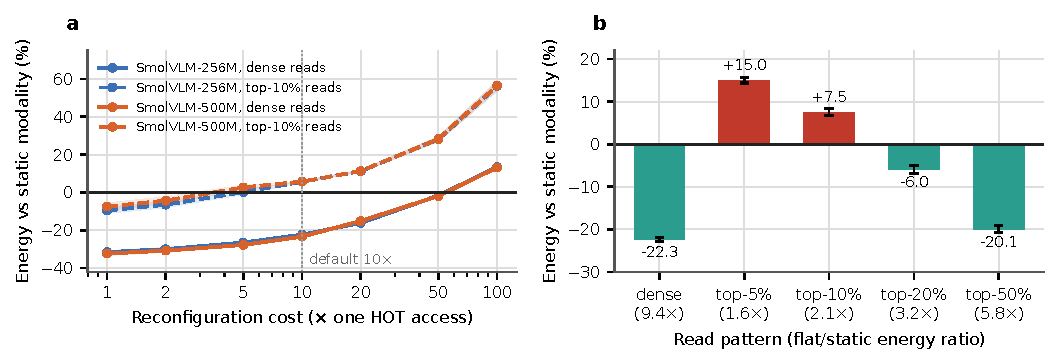
\includegraphics[width=\linewidth]{figs/fig_cost_sparse.pdf}
\caption{(a) Energy saving vs reconfiguration cost (thresholds re-selected per cost; bands are 95\% CIs); the saving breaks even near $50\times$. (b) Dense reads are required: the saving shrinks and reverses as reads become sparse (flat/static energy ratio in parentheses).}
\label{fig:cost}
\end{figure}

\textbf{Mechanism.} Ablating the policy at the selected 256M thresholds shows where the saving comes from (Fig.~\ref{fig:mech}): demote-only gives $-24.2\%$ energy but \emph{worsens} quality by $+6.8\%$; promote-only costs $+1.8\%$ energy and improves quality by $-7.6\%$; the full policy gives $-22.3\%$ energy and $-0.8\%$ quality. \textbf{Demotion earns the energy; promotion buys back the quality it would otherwise give up.} 87\% of moves (1008 of 1156 per session) are on prompt-text entries, consistent with E4. A min-dwell requirement only trades saving for fewer moves ($0/5/20/40$ steps: $-22.3/-19.8/-13.8/-5.9\%$), so the default no-dwell policy is preferred.

\begin{figure}[t]
\centering
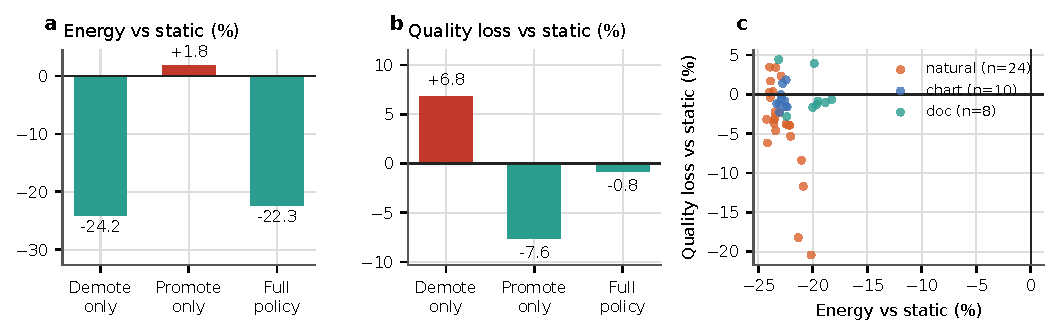
\includegraphics[width=\linewidth]{figs/fig_mech.pdf}
\caption{Mechanism ablation on 256M at the selected thresholds (a, b), and the per-trace outcome of the full policy by image kind (c): all 42 points have negative energy change; quality scatters around zero.}
\label{fig:mech}
\end{figure}

\textbf{What E5 left open.} Two objections that no amount of further scaling answers: (1) the policy consumed the \emph{true} attention of every entry for free; (2) ``quality'' is an attention-weighted error proxy, not a measurement of what the model says. The next two experiments address them.

\subsection{E6 --- Objection 1: the policy used the true attention for free}
\label{sec:est}
\textbf{Question.} E3--E5 fed the importance monitor the exact attention weight of every (token, layer) entry at every step. A real system must compute, approximate or sample this signal. How much of the saving survives an imperfect one? \textbf{Setup.} An \emph{estimator} sits between the true weights and the monitor (Fig.~\ref{fig:arch}); quality and access energy are still charged with the \emph{true} weights, so the policy simply acts on a worse signal. We test seven degradations on the 42 256M traces with dense reads, $10\times$ cost and the same leave-one-out protocol (thresholds re-selected per estimator over a 10-configuration grid; the oracle row reproduces E5):
\begin{itemize}[leftmargin=1.2em]
\item \emph{Noise} $\sigma\in\{0.25,0.5,1\}$: each weight is multiplied by an independent log-normal factor (for $\sigma{=}1$, a factor within $e^{\pm1}$ for 68\% of reads and mean-inflated by $1.65\times$).
\item \emph{Sampled}: the monitor sees attention only every 2nd, 4th or 8th step (EMA decay raised to the same power to keep its time constant).
\item \emph{Stale}: the monitor sees the weights from 1 or 4 steps ago.
\item \emph{Token-shared}: one score per token, the mean over layers, shared by all of its entries, i.e.\ what a system obtains if it can afford only one importance value per token rather than one per (token, layer).
\item Two combinations (token-shared with 4-step sampling; noise $\sigma{=}0.5$ with 4-step sampling).
\end{itemize}

\begin{figure}[t]
\centering
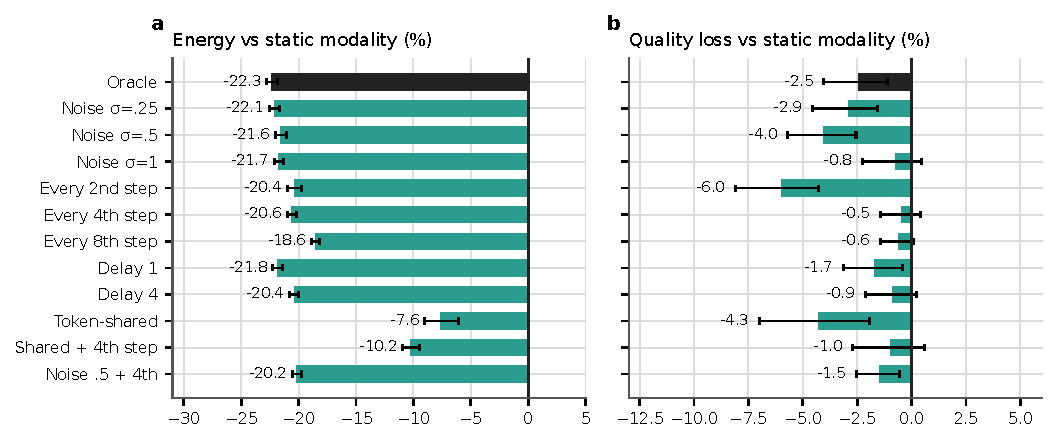
\includegraphics[width=0.93\linewidth]{figs/fig_estimators.pdf}
\caption{E6: held-out effect of the dynamic policy under imperfect importance signals (256M, 42 traces, dense reads, $10\times$; bars are leave-one-out means with bootstrap 95\% CIs; black = oracle). Per-entry signals can be noisy, sparse in time or stale and keep $\ge$18.6\% of the saving; a single score per token does not.}
\label{fig:est}
\end{figure}

\textbf{Finding 1: the saving is robust to a degraded per-entry signal.} Noise up to $\sigma{=}1$ leaves $-21.8\%$ energy (oracle $-22.3\%$); observing attention only every 8th step gives $-18.6\%$, a signal delayed by 4 steps gives $-20.4\%$, and noise plus 4-step sampling gives $-20.2\%$ (Fig.~\ref{fig:est}). All of these meet the pre-specified criterion (energy saving $\ge10\%$, quality change $\le+2\%$, CI excluding 0). Quality does not degrade: it stays at or below the static baseline (between $-6.0\%$ and $-0.5\%$), because a noisier or older signal promotes slightly more entries. The number of moves is essentially unchanged (1111--1298 against 1190 for the oracle). \textbf{Because the saving equals the energy a system may spend on estimation, the oracle's 22.3\% of static access energy is also the upper bound on the estimator's own cost per session}, and a signal sampled every 4th step still leaves $\sim$20\% of headroom.

\textbf{Finding 2: the signal must stay per (token, layer).} Collapsing importance to one score per token cuts the saving to $-7.6\%$ [$-9.0,-6.1$] (with 4-step sampling, $-10.2\%$), below the 10\% criterion. At the oracle's thresholds the token-shared signal reaches $-18.7\%$ energy but loses $+12.8\%$ quality, so the policy cannot find an operating point as good as the per-entry one. This is the same lesson as E4, seen from the signal side: what the policy exploits is variation \emph{between layers of the same token}, not a per-token summary. \textbf{Caveat.} All estimators here are free; we charge no energy or latency for producing them, and do not model any specific approximate scorer (e.g.\ low-precision or sampled key scores). E6 shows how imperfect the signal may be, not what a concrete estimator costs.

\subsection{E7 --- Objection 2: is the quality proxy real?}
\label{sec:real}
\textbf{Question.} Everything so far scores quality with $\epsilon\times$(attention mass served from \warm{}). Does a policy that the proxy ranks better also change the real model's output less when INT4 is actually applied? \textbf{Setup.} For each of the 42 images, we replay each policy's placement on the real SmolVLM-256M. The simulator logs, for every decode step, which (token, layer) entries are in \warm{}; the model is then teacher-forced on its own full-precision 64-token generation, and at step $t$ the cached K and V of exactly those entries are replaced by their INT4 round trip (per-token asymmetric min-max, groups of 32). We measure the KL divergence $\mathrm{KL}(p_{\text{full}}\,\|\,p_{\text{policy}})$ of the next-token distribution (mean over the 64 steps) and top-1 agreement with the full-precision model. The replay reproduces the saved generation on all 42 images. Four placements are compared: static modality, the dynamic policy (selected thresholds 8/0.4), \emph{random placement with the same number of INT4 entries at every step as the dynamic policy} (a control for \emph{which} entries are demoted), and everything in INT4.

\begin{figure}[t]
\centering
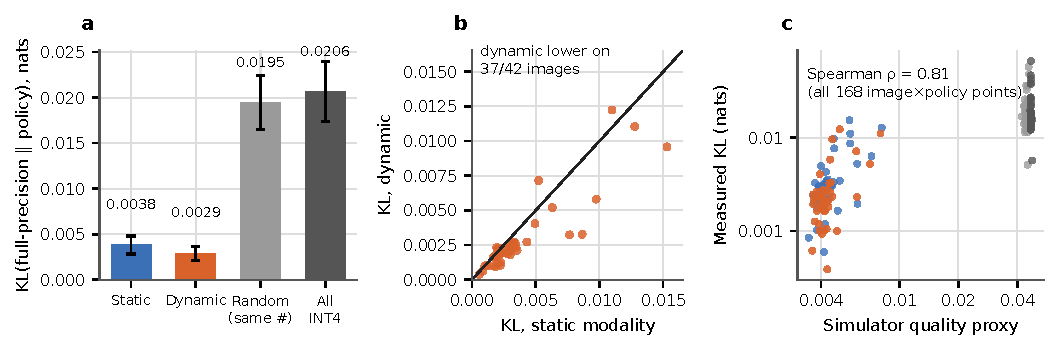
\includegraphics[width=\linewidth]{figs/fig_real_output.pdf}
\caption{E7: real output change under INT4 placement, 42 images, SmolVLM-256M. (a) Mean KL to the full-precision model (95\% CIs). (b) Dynamic vs static per image: points below the diagonal favour the dynamic policy. (c) The simulator's quality proxy against measured KL for all 168 (image, policy) points.}
\label{fig:real}
\end{figure}

\begin{table}[t]
\centering\small
\caption{E7: measured effect of INT4 placement on the next-token distribution (mean over 42 images). Fraction of entries in INT4 is the mean over steps.}
\label{tab:e7}
\begin{tabular}{lcccc}
\toprule
Placement & INT4 entries & KL (nats) & Top-1 agreement & Proxy $\epsilon\!\cdot\!$mass\\
\midrule
Static modality               & 91.8\% & 0.00382 & 0.976 & 0.0045\\
Dynamic (ours)                & 94.9\% & \textbf{0.00291} & 0.977 & 0.0044\\
Random, same INT4 count       & 94.9\% & 0.01946 & 0.930 & 0.0445\\
All INT4                      & 100\%  & 0.02064 & 0.929 & 0.0468\\
\bottomrule
\end{tabular}
\end{table}

\textbf{Finding 1: the policy picks the right entries.} The dynamic policy places \emph{more} entries in INT4 than static modality (94.9\% vs 91.8\%) and still changes the output distribution \textbf{21.8\% less} (per-image mean, 95\% CI $[15.3,28.1]\%$; lower on 37 of 42 images: 22/24 natural, 9/10 chart, 6/8 document). Random placement with the same INT4 count is \textbf{9.4$\times$} worse than the dynamic policy ($[7.8,11.1]\times$; worse on all 42 images) and indistinguishable from putting everything in INT4. The energy saving of E5 is therefore not obtained by demoting entries at random, and the entries the policy keeps in \hot{} are the ones the real model is sensitive to.

\textbf{Finding 2: the proxy is a usable but conservative guide.} Across all 168 points the proxy and the measured KL are strongly rank-correlated (Spearman $\rho{=}0.81$; Pearson on log scale 0.88), mostly because the proxy separates policies that demote important entries from those that do not (Fig.~\ref{fig:real}c). Within the static/dynamic pair the correlation is weaker ($\rho{=}0.49$), the proxy's per-image sign of the dynamic-vs-static difference matches the measured one on 29 of 42 images, and it \emph{understates} the advantage: the proxy predicts $-2.5\%$, the measurement $-21.8\%$. Top-1 agreement does not separate dynamic from static (difference $+0.1$ points, CI includes 0). \textbf{Caveats.} The effects of INT4 on this small model are small in absolute terms (even all-INT4 keeps 93\% top-1 agreement over 64 teacher-forced steps), so E7 validates the \emph{ordering and mechanism} rather than a task-accuracy claim, covers one model and the single INT4 scheme measured in Sec.~3.2, and uses KL as the quality measure, not a benchmark score.


\subsection{E8 --- Objection 3: where should each read run? Computation placement under contention}
\label{sec:e8}
\textbf{Question.} E1--E7 chose where data live, and the tier implied where a read was computed, with latencies summed serially. A memory-centric design must also decide \emph{where the computation runs} when compute units are finite and share a data path. Does the compute-site decision matter, and does the data-placement result survive contention? \textbf{Setup.} The system model of Sec.~\ref{sec:sys}, dense (reusable) reads, 42 traces on SmolVLM-256M. Policies: flat, static modality, and the dynamic policy at the E5 thresholds ($8\times/0.4\times$, \emph{not} re-tuned) with the bottom-up migration cost. Schedulers: \texttt{tier} (\warm{} reads run in memory), \texttt{host} (\warm{} is compressed storage; every read runs on the host) and \texttt{adaptive}. CIM capacity is swept from 2 to 64 units; 8 bus channels and 8 host lanes are fixed. Hypotheses and pass criteria H8a--H8c were written in the lab notes after the runs were launched but before any result was inspected (apart from one smoke-test trace). Values are means over traces of per-trace ratios to flat (the trace-to-trace s.d.\ of every ratio is below 0.01 for energy and below 0.04 for makespan).

\begin{figure}[t]
\centering
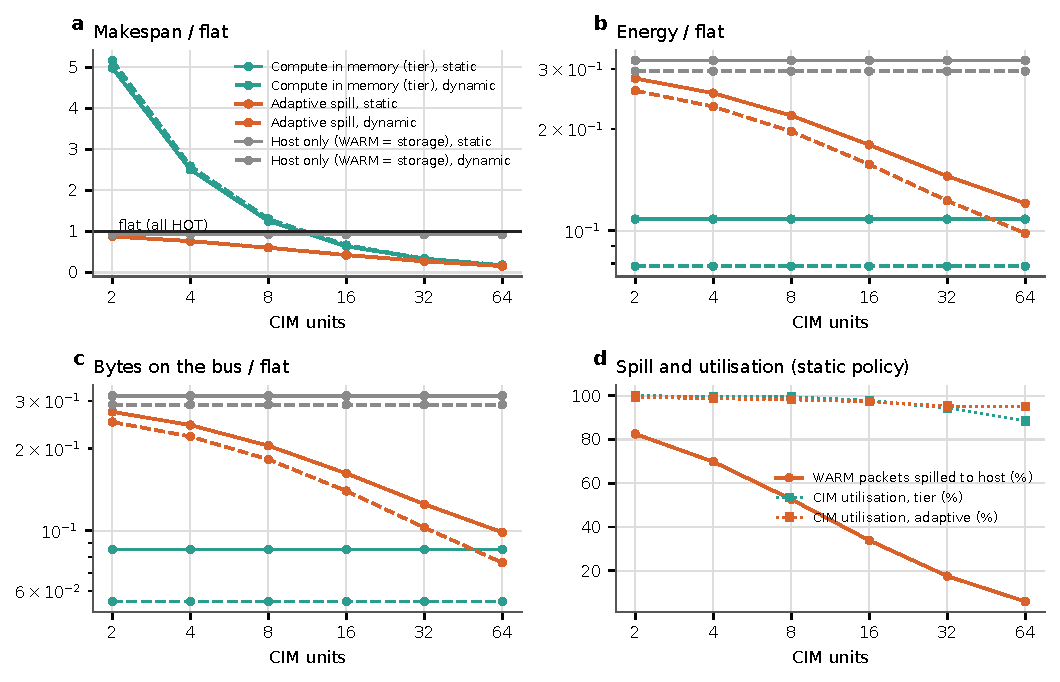
\includegraphics[width=\linewidth]{figs/fig_e8.pdf}
\caption{E8: compute-site scheduling vs CIM capacity (dense reads, 42 traces; solid = static modality, dashed = dynamic). (a) Makespan relative to flat: compute-in-memory alone is slower than flat below $\sim$16 units; host-only is capacity-independent; adaptive spill beats both. (b) Energy and (c) bytes on the bus relative to flat. (d) Fraction of \warm{} packets the adaptive scheduler spills to the host, and CIM utilisation.}
\label{fig:e8}
\end{figure}

\textbf{H8a --- contention reverses the serial-latency penalty: confirmed.} With 16 CIM units, static modality moves $11.8\times$ fewer bytes over the bus than flat, uses $9.3\times$ less energy and has a \emph{lower} makespan ($0.64\times$ flat's). Flat is bus-bound (99\% bus utilisation); static modality is CIM-bound (98\%). In the serialised model of E1--E7 the same placement looked $\sim$34\% \emph{slower} than flat, because serialisation forbids overlapping the two tiers. Part of what E1--E7 called a latency cost of tiering was an artefact of the cost model.

\textbf{H8b --- the compute-site decision is first-order: confirmed.} If \warm{} reads always run in memory, the verdict depends on CIM capacity: static modality is $5.0\times$, $2.5\times$ and $1.25\times$ \emph{slower} than flat with 2, 4 and 8 units, and breaks even near 16 (Fig.~\ref{fig:e8}a). The opposite extreme, treating \warm{} as compressed storage computed on the host, is capacity-independent ($0.92\times$ flat's makespan) but gives up most of the benefit: energy $0.319$ of flat versus $0.108$, and bytes on the bus $0.313$ versus $0.085$ (Fig.~\ref{fig:e8}b,c). The adaptive scheduler is better on makespan than \emph{both} at every capacity (e.g.\ $0.42\times$ flat at 16 units, against $0.64\times$ and $0.92\times$), because it keeps the CIM units and the host lanes busy at once; it spills 83\% of \warm{} packets at 2 units and 6\% at 64 (Fig.~\ref{fig:e8}d). The price is energy: at 16 units adaptive uses $1.66\times$ the energy of in-memory compute ($0.179$ vs $0.108$ of flat) for a $33\%$ lower makespan, still far below host-only ($0.319$). Compute placement is therefore a latency--energy trade-off that the runtime resolves from queue state, not a property of the tier.

\textbf{H8c --- data-placement gains survive contention: confirmed, with a latency cost.} At 16 CIM units with in-memory compute, the dynamic policy lowers energy by \textbf{27.4\%} against static modality (95\% CI $[27.0,27.8]$; larger than E5's $-22.3\%$ because the bottom-up migration costs $\approx\!1.05$ rather than $10$ \hot{} accesses) and bytes on the bus by $36\%$, at quality $2.5\%$ better. It is $4.7\%$ ($[4.6,4.9]$) \emph{slower} in makespan, plausibly because it keeps more entries on the host-side path and its 1.1k moves per session compete for the bus (we did not isolate the two). Under the adaptive scheduler the energy advantage over static shrinks to $12.5\%$ at 16 units and to $8.0\%$ at 2: spilled reads cost the same on the host regardless of how \warm{} came to hold the data, so a scarce CIM tier dilutes what any tiering policy can save.

\textbf{What E8 left open.} All of E1--E8 read every entry every step (or the top-$k$ of it). The task statement's own example has data with different \emph{reuse}: re-read, streamed once, accessed at random. E9 tests whether placement should differ across them.

\subsection{E9 --- Objection 4: should placement differ for reusable, streamed and randomly accessed data?}
\label{sec:e9}
\textbf{Question.} The same system may process a highly reusable dataset, a streaming dataset and a randomly accessed one. Everything up to E8 read each entry every step, so reuse was uniform. Does the best placement depend on the access regime, and can the runtime adapt without being told the regime? \textbf{Setup.} The three regimes of Sec.~\ref{sec:sys} (reusable = dense; random with 30\%, 10\% and 3\% of entries read per step; streaming = each entry read once), 42 traces, 16 CIM units, in-memory compute. Policies: static modality, the dynamic policy ($8\times/0.4\times$, not re-tuned for any regime) and the reuse-aware policy of Sec.~\ref{sec:sys}, each at the bottom-up migration cost and at $10\times$ that cost (a stress setting, equal to the cost assumed in E1--E7). Random draws use one seed per trace, so every policy sees the same reads. H9a--H9e were written down after the runs were launched and before any result was inspected.

\begin{table}[t]
\centering\small
\caption{E9: change against static modality (mean over 42 traces; energy and quality loss in \%, negative is better). ``Gate'' is the reuse-aware policy (the post-hoc variant of Sec.~\ref{sec:e9} is in Fig.~\ref{fig:e9}). Flat/static is the energy headroom of \warm{} in that regime.}
\label{tab:e9}
\setlength{\tabcolsep}{4pt}
\begin{tabular}{lcccccccc}
\toprule
 & Flat/ & \multicolumn{3}{c}{Dynamic, bottom-up cost} & \multicolumn{2}{c}{Dynamic, $10\times$} & \multicolumn{2}{c}{+ gate, $10\times$}\\
\cmidrule(lr){3-5}\cmidrule(lr){6-7}\cmidrule(lr){8-9}
Regime & static & Energy & Quality & Moves & Energy & Quality & Energy & Moves\\
\midrule
Reusable (dense)      & 9.3$\times$ & $-27.4$ & $-2.5$ & 1190 & $-21.6$ & $-2.5$ & $-21.6$ & 1190\\
Random, 30\% read     & 9.1$\times$ & $-25.1$ & $+3.9$ & 1038 & $-8.5$  & $+3.9$ & $-5.4$  & 744\\
Random, 10\% read     & 8.6$\times$ & $-15.8$ & $+5.7$ & 1064 & $+32.1$ & $+5.7$ & $+2.2$  & 91\\
Random, 3\% read      & 7.3$\times$ & $+2.1$  & $+2.6$ & 645  & $+81.9$ & $+2.6$ & $+1.1$  & 9\\
Streaming (read once) & 7.3$\times$ & $0$ & $0$ & 0 & $0$ & $0$ & $0$ & 0\\
\bottomrule
\end{tabular}
\end{table}

\begin{figure}[t]
\centering
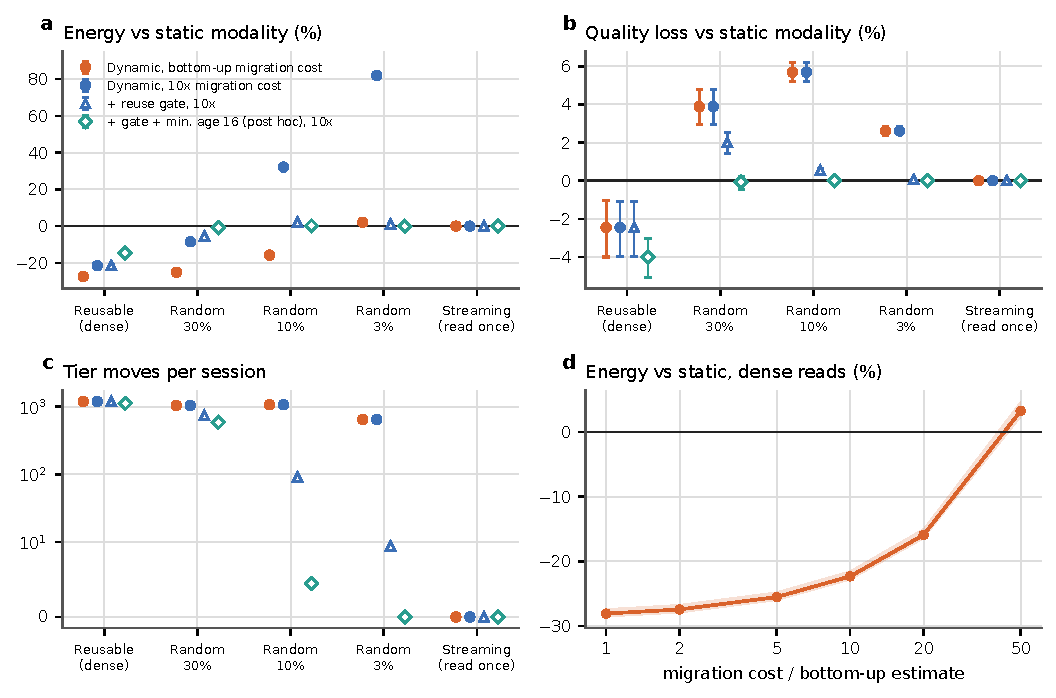
\includegraphics[width=\linewidth]{figs/fig_e9.pdf}
\caption{E9: (a) energy and (b) quality loss against static modality, by access regime (95\% CIs). (c) Tier moves per session. (d) Energy against migration cost in the dense regime (14 traces; band = 95\% CI): break-even near $45\times$ the bottom-up estimate. The green diamonds are the post-hoc variant.}
\label{fig:e9}
\end{figure}

\textbf{H9a, reusable data: confirmed.} Dynamic placement lowers energy by 27.4\% at the bottom-up cost (95\% CI $[26.9,27.8]$) and by 21.6\% at $10\times$ (E5's $-22.3\%$ in the first simulator), with quality 2.5\% better ($[1.1,4.0]$), 1190 moves per session, and a makespan penalty of 4.7\% and 13.1\% respectively.

\textbf{H9b, streaming data: confirmed, trivially.} With one read per entry, no entry is observed twice. The monitor's warm-up (Sec.~3.3) therefore never lets a move happen, and the dynamic and reuse-aware policies are identical to static modality in all metrics. The right decision for streamed data is simply the initial placement. The reason is worth stating because it is not a finding about the policy's cleverness: read-once data \emph{cannot repay} a migration, and the warm-up happens to encode that. (In this regime flat is 14\% \emph{faster} than static but uses $7.3\times$ the energy: the compute-site trade-off of E8 reappears with few reads.)

\textbf{H9c, random access: not confirmed as stated.} At $10\times$ migration cost the ungated dynamic policy is much worse than static when reads are sparse ($+32.1\%$ energy at 10\% reads, $+81.9\%$ at 3\%), because it pays $\sim$1000 moves per session for entries that are read too rarely to repay them. The gate removes most of the harm by suppressing 91\% and 98\% of those moves (1064$\to$91 and 645$\to$9) and brings the loss to $+2.2\%$ and $+1.1\%$, but our criterion was parity within 1\%, and the gate does \emph{not} meet it. With the bottom-up cost the break-even is only 1.08 reads, the gate never engages, and the dynamic policy saves energy under random access ($-15.8\%$ at 10\% reads, $-25.1\%$ at 30\%) \emph{but loses quality} ($+5.7\%$ and $+3.9\%$ against static; $+2.6\%$ at 3\%, where it also loses energy). Dynamic placement is therefore not regret-free under random access even when migration is cheap. Its thresholds were fitted to dense reads, and a monitor that only observes entries when they happen to be read is a plausible but untested cause.

\textbf{H9d, no single policy: half confirmed.} The best policy differs by regime: dynamic for reusable data, static for sparse random access (10\% and 3\%), either for streams. The second part (the reuse-aware policy never exceeds static by more than 2\% energy) fails narrowly: $+2.2\%$ at 10\% reads and $10\times$ cost.

\textbf{Post-hoc diagnosis of the residual (not part of the protocol).} After seeing H9c fail we asked why the gate still lets $\sim$90 moves through. A look at one trace (82 moves, 79 of them on prefill entries) suggested a noisy read-frequency estimate early in the session: an entry read a few times in its first steps looks highly reused. Requiring a minimum age before the estimate is trusted tests that explanation. With a minimum age of 16 steps the gate removes the residual at $10\times$: $+0.13\%$ energy ($[0.11,0.15]$) and neutral quality at 10\% reads, $0.0\%$ at 3\% (no moves), $-0.8\%$ at 30\%, with 4.5 moves per session at 10\%. The price is paid in the reusable regime, where delaying early moves cuts the saving from $-21.6\%$ to $-14.6\%$ (and $-27.4\%\to-20.0\%$ at the bottom-up cost). The choice matters: ages 4 and 8 leave $+2.15\%$ and $+1.06\%$. Because the variant was designed after seeing these test traces, with three ages tried, it is a diagnosis of where the regret comes from, not a tuned headline result.

\textbf{H9e, migration-cost sensitivity.} In the explicit model (dense reads, 14 traces, fixed thresholds) the saving is $-28.1\%$ at the bottom-up cost, $-25.5\%$ at $5\times$, $-22.3\%$ at $10\times$, $-15.9\%$ at $20\times$ and $+3.3\%$ at $50\times$ (CI $[+2.3,+4.7]$), a break-even near $45\times$ the bottom-up estimate, in agreement with E5's $\sim\!50\times$ from a different cost model. Migration traffic is 1\%, 8\%, 15\% and 31\% of total energy at $1\times$, $10\times$, $20\times$ and $50\times$, and the makespan penalty grows from $+4.6\%$ to $+47.6\%$: with a shared bus, migrations cost time as well as energy.

\begin{table}[t]
\centering\small
\caption{Pre-specified hypotheses of E8--E9 and their outcome.}
\label{tab:score}
\begin{tabular}{>{\raggedright\arraybackslash}p{1.0cm}>{\raggedright\arraybackslash}p{10.2cm}>{\raggedright\arraybackslash}p{3.8cm}}
\toprule
 & Statement (abbreviated) & Outcome\\
\midrule
H8a & Tiering moves $\ge$5$\times$ fewer bytes and uses $\ge$5$\times$ less energy than flat, at lower makespan & Confirmed ($11.8\times$, $9.3\times$, $0.64\times$)\\
H8b & Compute site matters: in-memory-only slower than flat at $\le$4 CIM units; adaptive within 10\% of the better pure strategy, cheaper than host-only & Confirmed (adaptive better than both)\\
H8c & Dynamic $\ge$10\% lower energy than static under contention, quality within $+2\%$ & Confirmed ($-27.4\%$, $-2.5\%$); $+4.7\%$ makespan\\
H9a & Reusable: dynamic $\ge$10\% lower energy, neutral quality & Confirmed ($-27.4\%$ / $-21.6\%$)\\
H9b & Streaming: dynamic $\approx$ static & Confirmed (identical; no moves)\\
H9c & Random, $10\times$ cost: ungated dynamic loses; gated within $+1\%$ of static & Ungated loses; \textbf{gate misses} ($+2.2\%$, $+1.1\%$)\\
H9d & Best policy differs by regime; gated never $>2\%$ worse than static & Half: differs; \textbf{misses} narrowly ($+2.2\%$)\\
H9e & Break-even migration cost (reported) & $\approx$45$\times$ the bottom-up estimate\\
\bottomrule
\end{tabular}
\end{table}

\textbf{What E8--E9 establish.} Computation placement is a first-order decision (a wrong default is $5\times$ slower than no tiering at 2 CIM units); a runtime that watches queue state beats both fixed choices on makespan; and whether dynamic \emph{data} placement pays depends on reuse: strongly for reusable data, not at all for streams, and under random access only if migrations are priced against the reuse the runtime has observed. The reuse-aware policy removes most but, as pre-specified, not all of the regret under random access.


\section{Discussion}
\paragraph{What is established.} For dense per-layer reads, under one stylised but fixed cost model, importance-driven placement beats the strong static-modality baseline by $\sim$22--23\% energy at neutral quality on two model sizes and three image kinds, with thresholds that transfer across sizes and a break-even reconfiguration cost about five times the default. The saving is produced by demoting individual prompt-text entries whose importance is low \emph{in this prompt}, and the promotions that give quality back are few. The two added checks narrow the main objections: the gain does not require an oracle (it survives noisy, stale or sampled importance, provided importance stays per (token, layer)), and it is not an artefact of the quality proxy (when INT4 is applied in the real model, the policy keeps in \hot{} the entries that matter: its output divergence is 21.8\% below static modality's and 9.4$\times$ below random placement's). They do not replace hardware measurement, and neither the estimator's own cost nor a concrete approximate scorer is modelled. Under explicit resources (E8) the result holds and is stronger than in the serial model ($-27.4\%$ at the bottom-up migration cost, with $11.8\times$ fewer bytes on the bus than flat), but the compute-site decision it rests on is first-order: with scarce CIM units, computing every \warm{} read in memory is up to $5\times$ slower than not tiering at all, and a scheduler that spills to the host is better than either fixed choice. Whether data placement should be dynamic depends on reuse (E9).

\paragraph{Where it does not apply.} (i) Sparse reads: with top-10\% reads the policy is a net loss and the \hot{}/\warm{} headroom itself shrinks to $\sim$2$\times$. (ii) Reconfiguration costs above roughly $50\times$ a \hot{} access. (iii) Coarse-grained placement: a static layer or role map cannot reproduce the effect. (iv) Read-once (streamed) data: nothing can repay a migration and the right decision is the initial placement. (v) Sparsely and randomly read data: the dynamic policy is not regret-free even at the bottom-up migration cost (quality $+3.9$ to $+5.7\%$ against static at 30\% and 10\% reads), and at $10\times$ it loses up to $+82\%$ energy; a reuse gate removes most but not all of that. These boundaries are as much a part of the finding as the saving.

\paragraph{Why the negative results stayed in.} E2 and E4 overturned beliefs we held (that the synthetic trade-off was general; that the win was a layer effect). Keeping them is what makes the later claim credible: the scale-up in E5 was designed to be able to fail, and the criterion was fixed beforehand.

\paragraph{Limitations.}
\begin{itemize}[leftmargin=1.2em]
\item \textbf{Stylised cost model.} \warm{} is $10\times$ cheaper per byte and $1.5\times$ slower than \hot{}; the reconfiguration multiplier is swept but these ratios are not. Results are ratios between policies under shared assumptions, not device energies. There is no hardware measurement.
\item \textbf{Models and data.} Two sizes of one model family, 42 images, 64 decode steps, one prompt per image. Larger models (we planned SmolVLM-2.2B and dropped it), other families and long-form generation are untested. Attention is head-averaged per layer; per-head entries are not modelled.
\item \textbf{Two tiers, simple resources.} No capacity pressure on \hot{}. Contention exists only in E8--E9 (E1--E7 serialise latency) and is a small model: fixed counts of bus channels, host lanes and CIM units (only CIM is swept), FIFO queues, a per-step barrier, migrations that do not overlap reads, and a greedy scheduler with a work-conserving finish-time estimate. Bank conflicts, row-buffer behaviour, refresh and a real CIM array's constraints are not modelled.
\item \textbf{Access regimes are overlays.} The streaming and random regimes re-read the same real attention rows under a different read pattern; they are not separate real workloads. One query per image, decode only, no batching, no prefill cost.
\item \textbf{Scope of the two added checks.} E6 charges nothing for computing the importance signal. E7 covers one model, one INT4 scheme (the one measured in Sec.~3.2) and measures distributional change (KL over 64 teacher-forced steps), not benchmark accuracy; INT4 effects on this small model are small in absolute terms.
\item \textbf{Post-hoc choices} (logged above): the damping rule in E1, the threshold normalisation in E2, the grid widening in E5, the minimum-age variant in E9. The migration cost in E8--E9 is derived bottom-up from the same stylised tier table, so it is internally consistent but not a hardware measurement.
\end{itemize}

\section{Conclusion}
We asked where the computation on a multimodal KV cache should run, and answered with a chain of nine experiments in which every step confirmed or overturned the last. Dynamic, importance-driven placement of data between a conventional tier and a compute-in-memory tier pays off by $\sim$22--27\% energy at neutral quality when data are reused, for as long as migration costs less than about $45$--$50\times$ a conventional access, and it survives imperfect importance estimates and real INT4 error in the model. Under explicit shared resources the decision of \emph{where each read is computed} is as important as where data live: a wrong default is up to $5\times$ slower than no tiering, and a scheduler that watches queues and spills to the host is better than either fixed choice. Streamed data need no dynamic placement, and sparsely or randomly read data make dynamic placement a liability unless migrations are priced against observed reuse, which our reuse gate does only in part. The study also leaves a usable method: fix hypotheses and pass criteria before looking, report held-out numbers with intervals, say plainly which pre-specified criteria failed, and keep the experiments that did not work.

\paragraph{Reproducibility.} All code, traces, per-simulation CSVs and this paper's figure scripts are in the repository. \texttt{experiments/run\_m7.py}, \texttt{analyze\_m7.py}, \texttt{run\_m7\_estimators.py}, \texttt{validate\_real\_output.py} and \texttt{paper/make\_figures.py} regenerate Sections 5.5--5.7, and \texttt{src/kvtier/system.py}, \texttt{experiments/run\_m9.py} and \texttt{analyze\_m9.py} (E8--E9; 3,402 simulations, about 25 minutes on 7 cores); the lab notebook \texttt{NOTES.md} records every deviation chronologically.

\begin{thebibliography}{99}\small
\bibitem{vlcache} Tu, D., et al.: VL-Cache: Sparsity and modality-aware KV cache compression for vision-language model inference acceleration. arXiv (2024).
\bibitem{zipvl} He, E., et al.: ZipVL: Efficient large vision-language models with dynamic token sparsification. arXiv (2024).
\bibitem{aircache} Huang, K., et al.: AirCache: Activating inter-modal relevancy KV cache compression for efficient large vision-language model inference. arXiv (2025).
\bibitem{topv} Yang, C., et al.: TopV: Compatible token pruning with inference time optimization for fast and low-memory multimodal vision language model. CVPR (2025).
\bibitem{fastv} Chen, L., et al.: An image is worth 1/2 tokens after layer 2: Plug-and-play inference acceleration for large vision-language models. ECCV (2024).
\bibitem{h2o} Zhang, Z., et al.: H2O: Heavy-hitter oracle for efficient generative inference of large language models. NeurIPS (2023).
\bibitem{snapkv} Li, Y., et al.: SnapKV: LLM knows what you are looking for before generation. NeurIPS (2024).
\bibitem{streaming} Xiao, G., et al.: Efficient streaming language models with attention sinks. ICLR (2024).
\bibitem{kivi} Liu, Z., et al.: KIVI: A tuning-free asymmetric 2bit quantization for KV cache. ICML (2024).
\bibitem{quest} Tang, J., et al.: Quest: Query-aware sparsity for efficient long-context LLM inference. ICML (2024).
\bibitem{vllm} Kwon, W., et al.: Efficient memory management for large language model serving with PagedAttention. SOSP (2023).
\bibitem{mutlu19} Mutlu, O., Ghose, S., G\'omez-Luna, J., Ausavarungnirun, R.: Processing data where it makes sense: Enabling in-memory computation. Microprocessors and Microsystems 67 (2019).
\bibitem{hbmpim} Lee, S., et al.: Hardware architecture and software stack for PIM based on commercial DRAM technology. ISCA (2021).
\bibitem{attacc} Park, J., et al.: AttAcc! Unleashing the power of PIM for batched transformer-based generative model inference. ASPLOS (2024).
\bibitem{neupims} Heo, G., et al.: NeuPIMs: NPU-PIM heterogeneous acceleration for batched LLM inferencing. ASPLOS (2024).
\bibitem{smolvlm} Marafioti, A., et al.: SmolVLM: Redefining small and efficient multimodal models. arXiv (2025).
\bibitem{coco} Lin, T.-Y., et al.: Microsoft COCO: Common objects in context. ECCV (2014).
\end{thebibliography}


\appendix
\section{Glossary}
\begin{description}[leftmargin=2.2cm,labelwidth=2cm,itemsep=1pt]
\item[KV cache] Per-layer keys and values of every token already processed, re-read at every decoding step.
\item[Entry] The KV pair of one (token, layer); the unit that is placed.
\item[\hot{} / \warm{}] Conventional FP16 DRAM/HBM tier with host compute / INT4 compute-in-memory tier (cheaper per byte, slower, lossy).
\item[CIM] Compute-in-memory: arithmetic done inside the memory array, so that only a partial result crosses the bus.
\item[Static modality] Baseline: visual entries in \warm{}, text entries in \hot{}, never moved.
\item[Dynamic policy] Promotes/demotes entries on a live importance EMA with hysteresis, paying for every move.
\item[Migration] A tier move: read source tier, requantise, write destination tier.
\item[Spill] A \warm{} read computed on the host instead of in memory.
\item[Makespan] Simulated time of the whole session with resource contention (E8--E9); E1--E7 report serial latency.
\item[Reuse rate] Fraction of steps in which an entry was read; the gate in E9 extrapolates it to decide whether a migration will be repaid.
\item[KL] $\mathrm{KL}(p_{\text{full}}\,\|\,p_{\text{policy}})$ of the next-token distribution, used in E7.
\end{description}

\section{Pre-specified hypotheses of E8--E9}
Written in the lab notes (\texttt{NOTES.md}, section M9) after the runs were launched and before any result was inspected, apart from one smoke-test trace. Thresholds are the E5 choice ($8\times/0.4\times$) throughout.
\begin{description}[leftmargin=1.1cm,labelwidth=0.9cm,itemsep=1pt]
\item[H8a] Static modality vs flat moves $\ge5\times$ fewer bus bytes and uses $\ge5\times$ less energy, and its makespan is \emph{lower} than flat's.
\item[H8b] At $\le4$ CIM units, always computing in memory makes static modality \emph{slower than flat}; the adaptive scheduler is within 10\% of the better of \{tier, host\} at every capacity and uses less energy than host-only.
\item[H8c] Dynamic vs static: $\ge10\%$ lower energy, quality loss within $+2\%$, at default resources and the bottom-up migration cost.
\item[H9a] Reusable (dense): dynamic beats static by $\ge10\%$ energy at neutral quality.
\item[H9b] Streaming: no move can be repaid; dynamic $\approx$ static (energy difference $<2\%$).
\item[H9c] Random access at $10\times$ cost: ungated dynamic is worse than static; the gated policy is within $+1\%$ of $\min$(static, ungated).
\item[H9d] The best of \{flat, static, dynamic, dynamic+gate\} differs across regimes, and dynamic+gate is never more than $2\%$ worse than static in energy.
\item[H9e] Break-even migration scale in the explicit model (reported; no threshold pre-set).
\end{description}
Outcomes are in Tab.~\ref{tab:score}: H9c and the second half of H9d were \emph{not} met.

\section{Full result tables}
\begin{table}[h]
\centering\scriptsize\setlength{\tabcolsep}{3.2pt}
\caption{E8 in full: per-trace ratios to flat, averaged over 42 traces, by CIM capacity. T = compute in memory (tier), H = host only, A = adaptive spill. Last column: share of \warm{} packets the adaptive scheduler spilled. Flat: mean makespan 5104 $\mu$s, mean energy 3681 $\mu$J.}
\label{tab:e8full}
\begin{tabular}{c ccc ccc ccc c}
\toprule
 & \multicolumn{3}{c}{Makespan / flat} & \multicolumn{3}{c}{Energy / flat} & \multicolumn{3}{c}{Bus bytes / flat} & \\
\cmidrule(lr){2-4}\cmidrule(lr){5-7}\cmidrule(lr){8-10}
CIM units & T & H & A & T & H & A & T & H & A & Spill (A)\\
\midrule
\multicolumn{11}{l}{\textit{Static modality}}\\
2 & 4.984 & 0.923 & 0.875 & 0.108 & 0.319 & 0.282 & 0.085 & 0.313 & 0.273 & 83\%\\
4 & 2.504 & 0.923 & 0.762 & 0.108 & 0.319 & 0.255 & 0.085 & 0.313 & 0.244 & 70\%\\
8 & 1.252 & 0.923 & 0.601 & 0.108 & 0.319 & 0.219 & 0.085 & 0.313 & 0.205 & 53\%\\
16 & 0.637 & 0.923 & 0.424 & 0.108 & 0.319 & 0.179 & 0.085 & 0.313 & 0.162 & 34\%\\
32 & 0.330 & 0.923 & 0.270 & 0.108 & 0.319 & 0.145 & 0.085 & 0.313 & 0.125 & 18\%\\
64 & 0.176 & 0.923 & 0.154 & 0.108 & 0.319 & 0.121 & 0.085 & 0.313 & 0.098 & 6\%\\
\midrule
\multicolumn{11}{l}{\textit{Dynamic ($8\times/0.4\times$)}}\\
2 & 5.165 & 0.926 & 0.880 & 0.079 & 0.296 & 0.260 & 0.055 & 0.290 & 0.250 & 83\%\\
4 & 2.591 & 0.926 & 0.767 & 0.079 & 0.296 & 0.233 & 0.055 & 0.290 & 0.221 & 71\%\\
8 & 1.306 & 0.926 & 0.606 & 0.079 & 0.296 & 0.197 & 0.055 & 0.290 & 0.182 & 54\%\\
16 & 0.667 & 0.926 & 0.429 & 0.079 & 0.296 & 0.157 & 0.055 & 0.290 & 0.140 & 36\%\\
32 & 0.338 & 0.926 & 0.275 & 0.079 & 0.296 & 0.123 & 0.055 & 0.290 & 0.103 & 20\%\\
64 & 0.184 & 0.926 & 0.160 & 0.079 & 0.296 & 0.098 & 0.055 & 0.290 & 0.076 & 9\%\\
\bottomrule
\end{tabular}
\end{table}

\begin{table}[h]
\centering\scriptsize\setlength{\tabcolsep}{3pt}
\caption{E9 in full: change against static modality (\%, mean over 42 traces, paired-bootstrap 95\% CI in brackets). Scale = migration cost relative to the bottom-up estimate. Moves per session; bus bytes and makespan as \% change; Win = fraction of traces with lower energy and quality loss at most 2\% worse. $^\dagger$ Post-hoc variants (see text); streaming rows for gated variants were not run (the dynamic policy makes no moves there).}
\label{tab:e9full}
\begin{tabular}{llcccccc}
\toprule
Policy & Scale & Energy & Quality loss & Moves & Bus bytes & Makespan & Win\\
\midrule
\multicolumn{8}{l}{\textit{Reusable (dense)}}\\
\quad Flat (headroom) & -- & 9.25$\times$ static & -- & -- & -- & -- & --\\
\quad Dynamic & 1$\times$ & -27.4 [-27.8, -27.0] & -2.5 [-4.0, -1.0] & 1190 & -35.6 & +4.7 & 0.88\\
\quad Dynamic & 10$\times$ & -21.6 [-22.0, -21.1] & -2.5 [-4.0, -1.1] & 1190 & -35.6 & +13.1 & 0.88\\
\quad + reuse gate & 1$\times$ & -27.4 [-27.8, -27.0] & -2.5 [-4.0, -1.0] & 1190 & -35.6 & +4.7 & 0.88\\
\quad + reuse gate & 10$\times$ & -21.6 [-22.0, -21.1] & -2.5 [-4.0, -1.1] & 1190 & -35.6 & +13.1 & 0.88\\
\quad + gate, min age 8$^\dagger$ & 1$\times$ & -23.1 [-23.6, -22.5] & -5.4 [-6.7, -4.3] & 1136 & -30.0 & +4.2 & 1.00\\
\quad + gate, min age 8$^\dagger$ & 10$\times$ & -17.5 [-18.0, -17.0] & -5.4 [-6.7, -4.2] & 1136 & -30.0 & +13.0 & 1.00\\
\quad + gate, min age 16$^\dagger$ & 1$\times$ & -20.0 [-20.5, -19.5] & -4.0 [-5.1, -3.0] & 1115 & -26.0 & +3.7 & 1.00\\
\quad + gate, min age 16$^\dagger$ & 10$\times$ & -14.6 [-15.0, -14.1] & -4.0 [-5.1, -3.0] & 1115 & -26.0 & +11.9 & 1.00\\
\midrule
\multicolumn{8}{l}{\textit{Random 30\%}}\\
\quad Flat (headroom) & -- & 9.07$\times$ static & -- & -- & -- & -- & --\\
\quad Dynamic & 1$\times$ & -25.1 [-25.4, -24.7] & +3.9 [+3.0, +4.8] & 1038 & -32.2 & +4.4 & 0.14\\
\quad Dynamic & 10$\times$ & -8.5 [-8.7, -8.3] & +3.9 [+2.9, +4.8] & 1038 & -32.2 & +44.0 & 0.14\\
\quad + reuse gate & 1$\times$ & -25.1 [-25.4, -24.7] & +3.9 [+3.0, +4.8] & 1038 & -32.2 & +4.4 & 0.14\\
\quad + reuse gate & 10$\times$ & -5.4 [-5.5, -5.2] & +2.0 [+1.4, +2.5] & 744 & -22.1 & +34.1 & 0.45\\
\quad + gate, min age 4$^\dagger$ & 1$\times$ & -24.9 [-25.2, -24.5] & +3.7 [+2.8, +4.6] & 1035 & -31.9 & +3.8 & 0.14\\
\quad + gate, min age 4$^\dagger$ & 10$\times$ & -5.2 [-5.3, -5.1] & +1.8 [+1.3, +2.4] & 741 & -21.8 & +28.0 & 0.48\\
\quad + gate, min age 8$^\dagger$ & 1$\times$ & -23.6 [-23.9, -23.2] & +2.8 [+2.0, +3.7] & 1021 & -30.2 & +2.9 & 0.29\\
\quad + gate, min age 8$^\dagger$ & 10$\times$ & -3.6 [-3.7, -3.5] & +0.7 [+0.2, +1.1] & 687 & -18.7 & +23.1 & 0.86\\
\quad + gate, min age 16$^\dagger$ & 1$\times$ & -19.6 [-19.9, -19.2] & +1.0 [+0.4, +1.6] & 983 & -25.0 & +1.5 & 0.71\\
\quad + gate, min age 16$^\dagger$ & 10$\times$ & -0.8 [-0.9, -0.7] & -0.1 [-0.5, +0.2] & 586 & -13.0 & +22.7 & 1.00\\
\midrule
\multicolumn{8}{l}{\textit{Random 10\%}}\\
\quad Flat (headroom) & -- & 8.58$\times$ static & -- & -- & -- & -- & --\\
\quad Dynamic & 1$\times$ & -15.8 [-16.0, -15.5] & +5.7 [+5.2, +6.2] & 1064 & -19.1 & +18.6 & 0.00\\
\quad Dynamic & 10$\times$ & +32.1 [+31.7, +32.6] & +5.7 [+5.2, +6.2] & 1064 & -19.1 & +186.2 & 0.00\\
\quad + reuse gate & 1$\times$ & -15.8 [-16.0, -15.5] & +5.7 [+5.2, +6.2] & 1059 & -19.1 & +18.5 & 0.00\\
\quad + reuse gate & 10$\times$ & +2.2 [+2.1, +2.2] & +0.5 [+0.4, +0.6] & 91 & -2.4 & +15.7 & 0.00\\
\quad + gate, min age 4$^\dagger$ & 1$\times$ & -15.8 [-16.0, -15.5] & +5.7 [+5.2, +6.2] & 1059 & -19.1 & +18.5 & 0.00\\
\quad + gate, min age 4$^\dagger$ & 10$\times$ & +2.1 [+2.1, +2.2] & +0.5 [+0.4, +0.6] & 91 & -2.4 & +15.5 & 0.00\\
\quad + gate, min age 8$^\dagger$ & 1$\times$ & -15.5 [-15.8, -15.3] & +5.5 [+5.1, +6.0] & 1057 & -18.8 & +16.4 & 0.00\\
\quad + gate, min age 8$^\dagger$ & 10$\times$ & +1.1 [+1.0, +1.1] & +0.1 [+0.1, +0.2] & 42 & -1.0 & +7.3 & 0.00\\
\quad + gate, min age 16$^\dagger$ & 1$\times$ & -14.3 [-14.5, -14.0] & +4.8 [+4.4, +5.2] & 1048 & -17.2 & +11.1 & 0.00\\
\quad + gate, min age 16$^\dagger$ & 10$\times$ & +0.1 [+0.1, +0.1] & +0.0 [-0.0, +0.0] & 4 & -0.1 & +0.8 & 0.00\\
\midrule
\multicolumn{8}{l}{\textit{Random 3\%}}\\
\quad Flat (headroom) & -- & 7.25$\times$ static & -- & -- & -- & -- & --\\
\quad Dynamic & 1$\times$ & +2.1 [+2.0, +2.2] & +2.6 [+2.4, +2.9] & 645 & +4.3 & +35.6 & 0.00\\
\quad Dynamic & 10$\times$ & +81.9 [+80.5, +83.3] & +2.6 [+2.4, +2.8] & 645 & +4.3 & +353.7 & 0.00\\
\quad + reuse gate & 1$\times$ & +1.5 [+1.4, +1.6] & +2.6 [+2.4, +2.8] & 598 & +3.4 & +33.0 & 0.00\\
\quad + reuse gate & 10$\times$ & +1.1 [+1.0, +1.2] & +0.1 [+0.0, +0.1] & 9 & -0.0 & +5.2 & 0.00\\
\quad + gate, min age 4$^\dagger$ & 1$\times$ & +1.5 [+1.4, +1.6] & +2.6 [+2.4, +2.8] & 598 & +3.4 & +33.0 & 0.00\\
\quad + gate, min age 4$^\dagger$ & 10$\times$ & +1.1 [+1.0, +1.2] & +0.1 [+0.0, +0.1] & 9 & -0.0 & +5.2 & 0.00\\
\quad + gate, min age 8$^\dagger$ & 1$\times$ & +1.5 [+1.4, +1.6] & +2.6 [+2.4, +2.8] & 598 & +3.5 & +33.0 & 0.00\\
\quad + gate, min age 8$^\dagger$ & 10$\times$ & +0.1 [+0.1, +0.2] & +0.0 [+0.0, +0.0] & 1 & -0.0 & +0.7 & 0.00\\
\quad + gate, min age 16$^\dagger$ & 1$\times$ & +1.7 [+1.6, +1.8] & +2.4 [+2.2, +2.7] & 596 & +3.6 & +30.7 & 0.00\\
\quad + gate, min age 16$^\dagger$ & 10$\times$ & +0.0 [+0.0, +0.0] & +0.0 [+0.0, +0.0] & 0 & +0.0 & +0.0 & 0.00\\
\midrule
\multicolumn{8}{l}{\textit{Streaming}}\\
\quad Flat (headroom) & -- & 7.28$\times$ static & -- & -- & -- & -- & --\\
\quad Dynamic & 1$\times$ & +0.0 [+0.0, +0.0] & +0.0 [+0.0, +0.0] & 0 & +0.0 & +0.0 & 0.00\\
\quad Dynamic & 10$\times$ & +0.0 [+0.0, +0.0] & +0.0 [+0.0, +0.0] & 0 & +0.0 & +0.0 & 0.00\\
\quad + reuse gate & 1$\times$ & +0.0 [+0.0, +0.0] & +0.0 [+0.0, +0.0] & 0 & +0.0 & +0.0 & 0.00\\
\quad + reuse gate & 10$\times$ & +0.0 [+0.0, +0.0] & +0.0 [+0.0, +0.0] & 0 & +0.0 & +0.0 & 0.00\\
\bottomrule
\end{tabular}
\end{table}


\section{Reproducing the results}
\begin{verbatim}
python -m venv .venv && .venv/bin/pip install -e ".[dev,vlm]"
.venv/bin/python -m pytest -q                       # 77 tests, incl. legacy-equivalence of system.py
.venv/bin/python experiments/make_dataset.py        # 42-image set (COCO photos re-downloaded)
.venv/bin/python experiments/extract_many.py        # real attention traces (MPS/GPU)
.venv/bin/python experiments/run_m7.py s256         # E5 grid, 256M      (analyze_m7.py for tables)
.venv/bin/python experiments/run_m7_estimators.py   # E6
.venv/bin/python experiments/validate_real_output.py 42 mps   # E7
.venv/bin/python experiments/run_m9.py e8 e9 e9b e9c          # E8-E9 (3,402 simulations)
.venv/bin/python experiments/analyze_m9.py          # summaries in results/m9_*_summary.csv
.venv/bin/python paper/make_figures.py && .venv/bin/python paper/make_tables.py
cd paper && pdflatex main.tex && pdflatex main.tex
\end{verbatim}
The simulations of E8--E9 take about 25 minutes on 7 cores; the lab notebook \texttt{NOTES.md} records every deviation and every pre-specified criterion in chronological order.

\end{document}
